% Options for packages loaded elsewhere
\PassOptionsToPackage{unicode}{hyperref}
\PassOptionsToPackage{hyphens}{url}
%
\documentclass[
]{book}
\usepackage{amsmath,amssymb}
\usepackage{lmodern}
\usepackage{iftex}
\ifPDFTeX
  \usepackage[T1]{fontenc}
  \usepackage[utf8]{inputenc}
  \usepackage{textcomp} % provide euro and other symbols
\else % if luatex or xetex
  \usepackage{unicode-math}
  \defaultfontfeatures{Scale=MatchLowercase}
  \defaultfontfeatures[\rmfamily]{Ligatures=TeX,Scale=1}
\fi
% Use upquote if available, for straight quotes in verbatim environments
\IfFileExists{upquote.sty}{\usepackage{upquote}}{}
\IfFileExists{microtype.sty}{% use microtype if available
  \usepackage[]{microtype}
  \UseMicrotypeSet[protrusion]{basicmath} % disable protrusion for tt fonts
}{}
\makeatletter
\@ifundefined{KOMAClassName}{% if non-KOMA class
  \IfFileExists{parskip.sty}{%
    \usepackage{parskip}
  }{% else
    \setlength{\parindent}{0pt}
    \setlength{\parskip}{6pt plus 2pt minus 1pt}}
}{% if KOMA class
  \KOMAoptions{parskip=half}}
\makeatother
\usepackage{xcolor}
\usepackage{color}
\usepackage{fancyvrb}
\newcommand{\VerbBar}{|}
\newcommand{\VERB}{\Verb[commandchars=\\\{\}]}
\DefineVerbatimEnvironment{Highlighting}{Verbatim}{commandchars=\\\{\}}
% Add ',fontsize=\small' for more characters per line
\usepackage{framed}
\definecolor{shadecolor}{RGB}{248,248,248}
\newenvironment{Shaded}{\begin{snugshade}}{\end{snugshade}}
\newcommand{\AlertTok}[1]{\textcolor[rgb]{0.94,0.16,0.16}{#1}}
\newcommand{\AnnotationTok}[1]{\textcolor[rgb]{0.56,0.35,0.01}{\textbf{\textit{#1}}}}
\newcommand{\AttributeTok}[1]{\textcolor[rgb]{0.77,0.63,0.00}{#1}}
\newcommand{\BaseNTok}[1]{\textcolor[rgb]{0.00,0.00,0.81}{#1}}
\newcommand{\BuiltInTok}[1]{#1}
\newcommand{\CharTok}[1]{\textcolor[rgb]{0.31,0.60,0.02}{#1}}
\newcommand{\CommentTok}[1]{\textcolor[rgb]{0.56,0.35,0.01}{\textit{#1}}}
\newcommand{\CommentVarTok}[1]{\textcolor[rgb]{0.56,0.35,0.01}{\textbf{\textit{#1}}}}
\newcommand{\ConstantTok}[1]{\textcolor[rgb]{0.00,0.00,0.00}{#1}}
\newcommand{\ControlFlowTok}[1]{\textcolor[rgb]{0.13,0.29,0.53}{\textbf{#1}}}
\newcommand{\DataTypeTok}[1]{\textcolor[rgb]{0.13,0.29,0.53}{#1}}
\newcommand{\DecValTok}[1]{\textcolor[rgb]{0.00,0.00,0.81}{#1}}
\newcommand{\DocumentationTok}[1]{\textcolor[rgb]{0.56,0.35,0.01}{\textbf{\textit{#1}}}}
\newcommand{\ErrorTok}[1]{\textcolor[rgb]{0.64,0.00,0.00}{\textbf{#1}}}
\newcommand{\ExtensionTok}[1]{#1}
\newcommand{\FloatTok}[1]{\textcolor[rgb]{0.00,0.00,0.81}{#1}}
\newcommand{\FunctionTok}[1]{\textcolor[rgb]{0.00,0.00,0.00}{#1}}
\newcommand{\ImportTok}[1]{#1}
\newcommand{\InformationTok}[1]{\textcolor[rgb]{0.56,0.35,0.01}{\textbf{\textit{#1}}}}
\newcommand{\KeywordTok}[1]{\textcolor[rgb]{0.13,0.29,0.53}{\textbf{#1}}}
\newcommand{\NormalTok}[1]{#1}
\newcommand{\OperatorTok}[1]{\textcolor[rgb]{0.81,0.36,0.00}{\textbf{#1}}}
\newcommand{\OtherTok}[1]{\textcolor[rgb]{0.56,0.35,0.01}{#1}}
\newcommand{\PreprocessorTok}[1]{\textcolor[rgb]{0.56,0.35,0.01}{\textit{#1}}}
\newcommand{\RegionMarkerTok}[1]{#1}
\newcommand{\SpecialCharTok}[1]{\textcolor[rgb]{0.00,0.00,0.00}{#1}}
\newcommand{\SpecialStringTok}[1]{\textcolor[rgb]{0.31,0.60,0.02}{#1}}
\newcommand{\StringTok}[1]{\textcolor[rgb]{0.31,0.60,0.02}{#1}}
\newcommand{\VariableTok}[1]{\textcolor[rgb]{0.00,0.00,0.00}{#1}}
\newcommand{\VerbatimStringTok}[1]{\textcolor[rgb]{0.31,0.60,0.02}{#1}}
\newcommand{\WarningTok}[1]{\textcolor[rgb]{0.56,0.35,0.01}{\textbf{\textit{#1}}}}
\usepackage{longtable,booktabs,array}
\usepackage{calc} % for calculating minipage widths
% Correct order of tables after \paragraph or \subparagraph
\usepackage{etoolbox}
\makeatletter
\patchcmd\longtable{\par}{\if@noskipsec\mbox{}\fi\par}{}{}
\makeatother
% Allow footnotes in longtable head/foot
\IfFileExists{footnotehyper.sty}{\usepackage{footnotehyper}}{\usepackage{footnote}}
\makesavenoteenv{longtable}
\usepackage{graphicx}
\makeatletter
\def\maxwidth{\ifdim\Gin@nat@width>\linewidth\linewidth\else\Gin@nat@width\fi}
\def\maxheight{\ifdim\Gin@nat@height>\textheight\textheight\else\Gin@nat@height\fi}
\makeatother
% Scale images if necessary, so that they will not overflow the page
% margins by default, and it is still possible to overwrite the defaults
% using explicit options in \includegraphics[width, height, ...]{}
\setkeys{Gin}{width=\maxwidth,height=\maxheight,keepaspectratio}
% Set default figure placement to htbp
\makeatletter
\def\fps@figure{htbp}
\makeatother
\setlength{\emergencystretch}{3em} % prevent overfull lines
\providecommand{\tightlist}{%
  \setlength{\itemsep}{0pt}\setlength{\parskip}{0pt}}
\setcounter{secnumdepth}{5}
\usepackage{booktabs}
\ifLuaTeX
  \usepackage{selnolig}  % disable illegal ligatures
\fi
\usepackage[]{natbib}
\bibliographystyle{plainnat}
\IfFileExists{bookmark.sty}{\usepackage{bookmark}}{\usepackage{hyperref}}
\IfFileExists{xurl.sty}{\usepackage{xurl}}{} % add URL line breaks if available
\urlstyle{same} % disable monospaced font for URLs
\hypersetup{
  pdftitle={Cystopteridaceae Phylogeny Project},
  pdfauthor={Chinedum Anajemba},
  hidelinks,
  pdfcreator={LaTeX via pandoc}}

\title{Cystopteridaceae Phylogeny Project}
\author{Chinedum Anajemba}
\date{2023-04-28}

\begin{document}
\maketitle

{
\setcounter{tocdepth}{1}
\tableofcontents
}
\hypertarget{overview}{%
\chapter*{Overview}\label{overview}}
\addcontentsline{toc}{chapter}{Overview}

\begin{figure}

{\centering 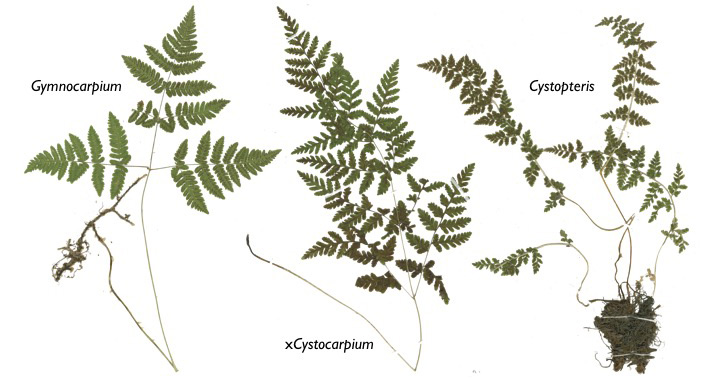
\includegraphics[width=1\linewidth]{img/Cystopteridaceae} 

}

\caption{Members of the Cystopteridaceae Family}\label{fig:image1}
\end{figure}

Welcome to my Cystopteridaceae Phylogeny Project!

The major goal of this project is to build a \textbf{species-level phylogeny} of the Cystopteridaceae ferns using nuclear gene loci from the most recognized species of the family. Cystopteridaceae is a family of small or medium-sized ferns that live in forests and crevices. The family contains 3 genera and about 50 species. This study provides more insight into the evolutionary relationship in the Cystopteridaceae family.
The content of this digital book is organized in the following Chapters:

Chapter \ref{data-assembly}: Data Assembly
Chapter \ref{database-design}: Database design and architecture
Chapter \ref{phasing-design}: Phasing of Gene Copies into Polyploid Subgenomes
Chapter \ref{phylogeny-design}: Species-level Phylogeny of Cystopteridaceae Ferns

The codes used in this analysis are available at \url{https://github.com/Chinedum335/Semester_Project}

\hypertarget{data-assembly}{%
\chapter{Data Assembly}\label{data-assembly}}

The sequence data used in this study were assembled using PURC (Pipeline for Untangling Reticulate Complexes). Allopolyploid species are polyploid species with more than two sets of chromosomes that originate from different species. Allopolyploids present a challenge for multilocus phylogenetic inference due to their multiple distinct subgenomes, each of which may have its own evolutionary history. Generating sequence data from allopolyploid lineages is challenging due to the difficulty in isolating the sequences of each of the distinct homoeologous gene copies. In addition, the phasing (assigning) of gene copies into their respective polyploid subgenomes remain another challenge even when the correct biological sequences are inferred. Recent advances in polyploid phylogenetics have made it possible to effectively undertake phylogenetic study of groups that comprise polyploids. PURC is a pipeline for inferring the underlying biological sequences (alleles, paralogs, or homeologs) from amplicon sequencing data (PacBio, Illumina, etc), de-multiplexing them (labeling each sequence with its locus and source sample), and cleaning them (removing PCR errors, sequencing errors, and chimeras). It is geared toward analyzing polyploid species complexes but is also effective for other applications; the final output of a full run includes an alignment for each locus with each homeolog or allele sequence in the amplicon data labeled with the source sample information and amount of coverage.

\begin{figure}

{\centering 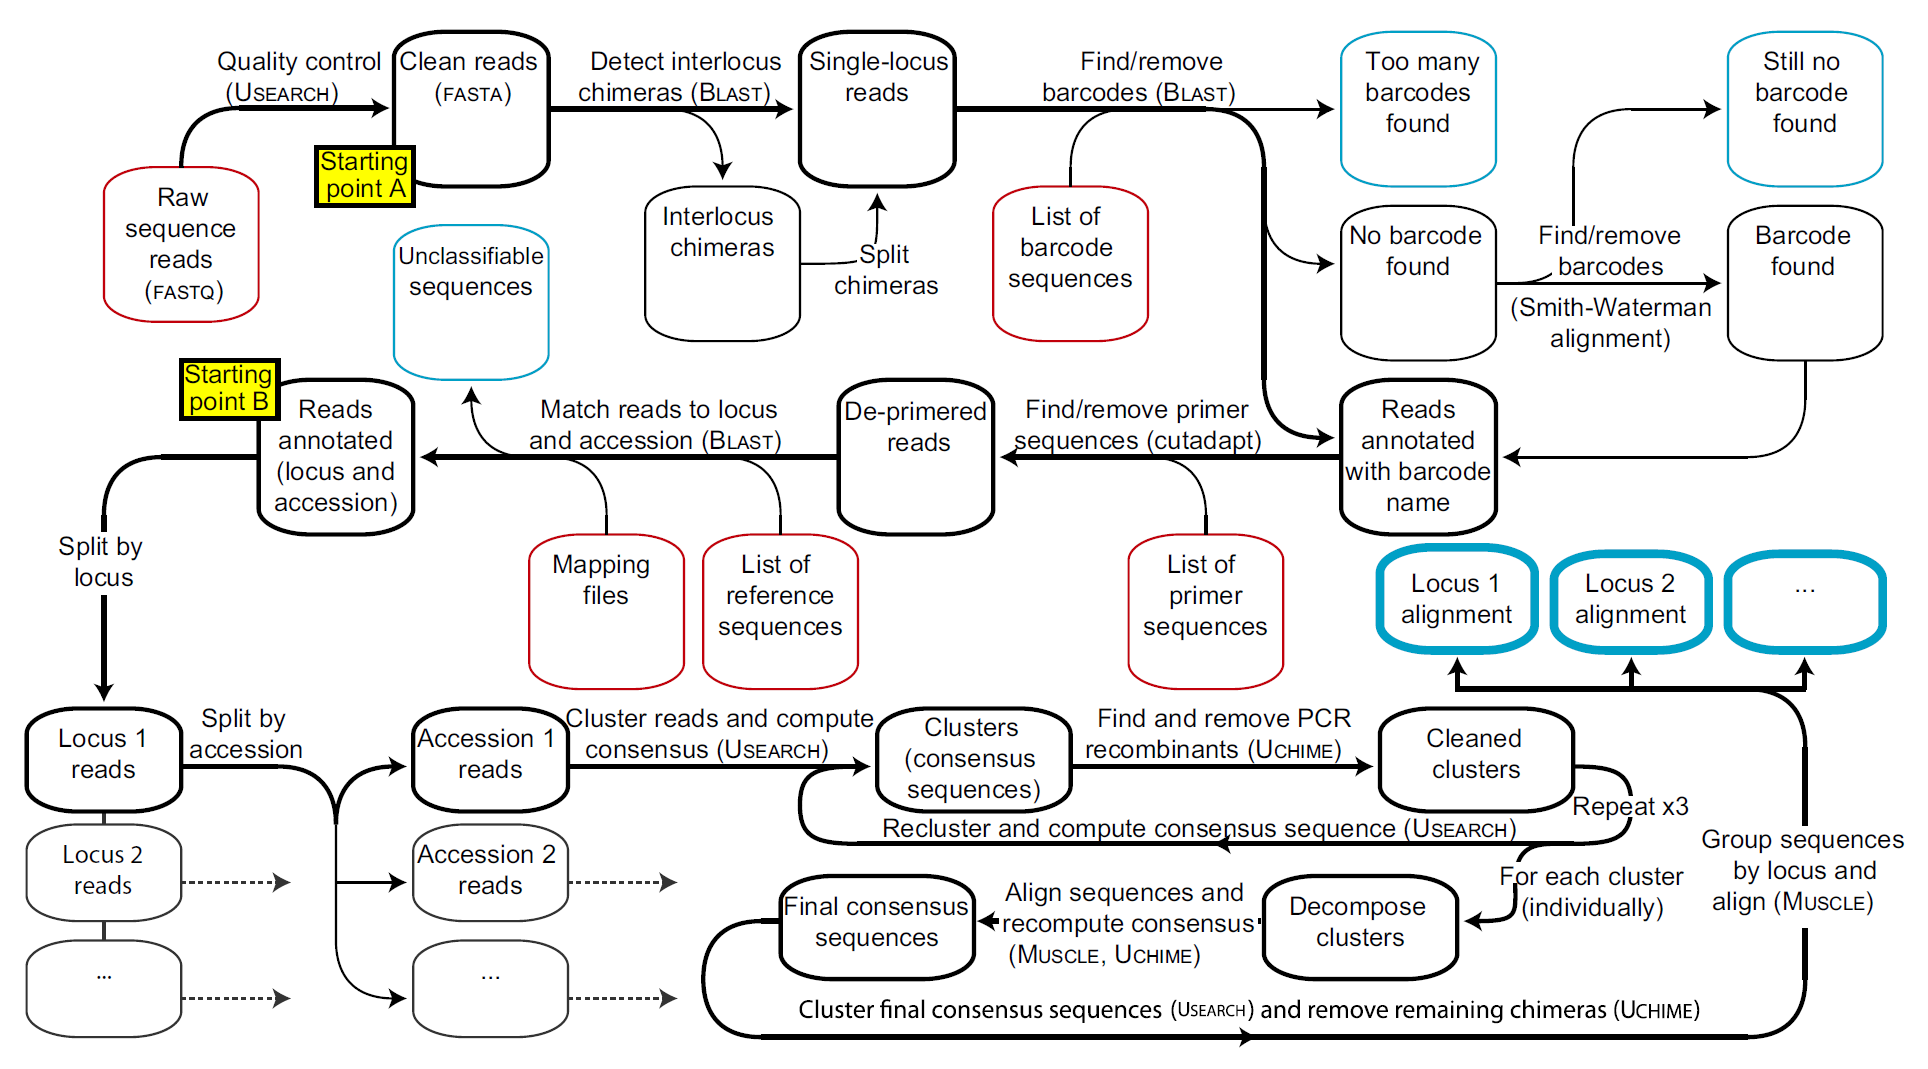
\includegraphics[width=1\linewidth]{img/purc} 

}

\caption{Pipeline for Untangling Reticulate Complexes}\label{fig:image3}
\end{figure}

In this study, I assembled the underlying sequences of four c.~1-kb-long nuclear loci from a sample of Cystopteridaceae accessions comprising 9 diploid species and 2 polyploid species using PURC.The reads of these sequences were generated using the PacBio platform.
A detailed instructions on PURC installation, how to prepare input files as well as additional information for troubleshooting can be found in the README file in the \href{https://bitbucket.org/peter_schafran/purc/}{PURC repository}

\hypertarget{database-design}{%
\chapter{Database design and architecture}\label{database-design}}

In this chapter, we will build a relational database that will translate real-world relationships between our data entities into structural relationships between our data tables. Let's take a look at the content and structure of the database:

\begin{figure}

{\centering 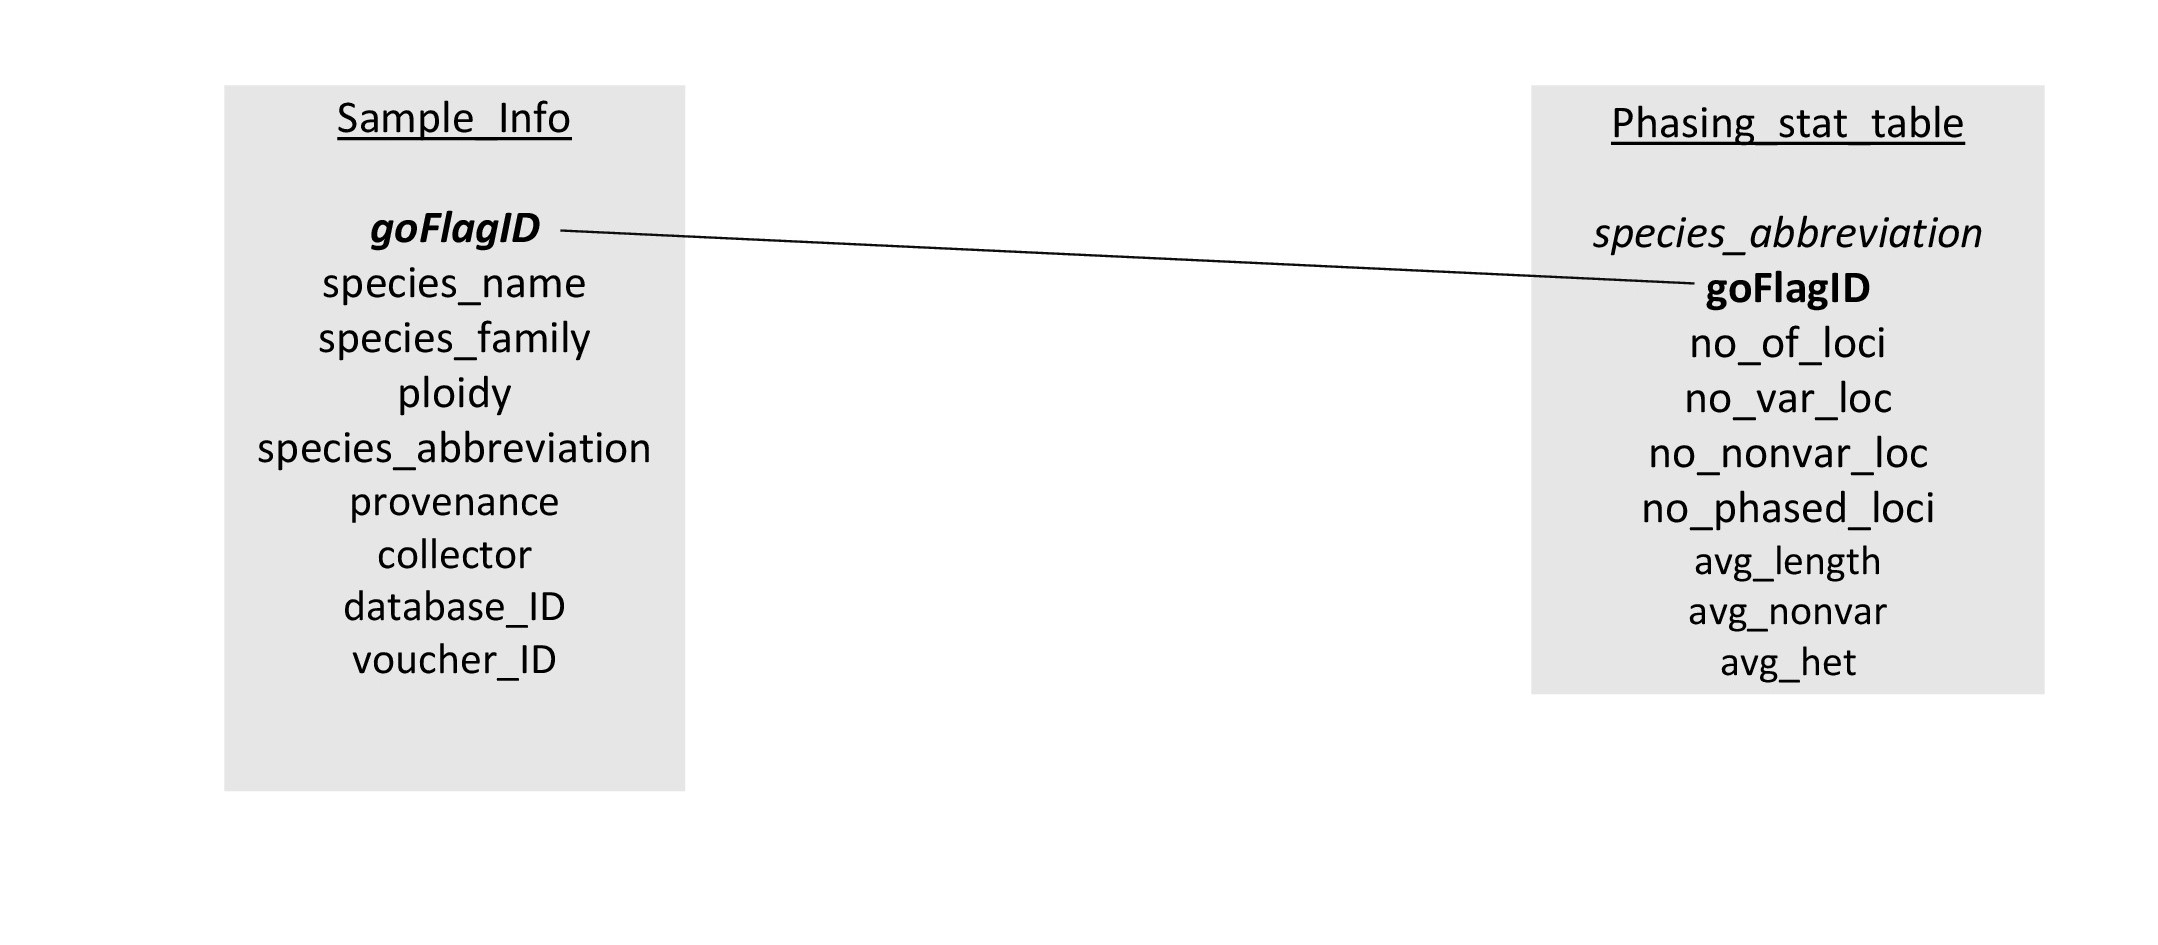
\includegraphics[width=1\linewidth]{img/SQL_database_image} 

}

\caption{Diagram of the cystpteridaceae database}\label{fig:image2}
\end{figure}

The database is composed of 2 tables- the sample\_Info and the phasing\_stat table. The sample\_info table includes individual information on the taxonomy, ploidy level and source of each species that are used in this project. The phasing statistics table provides the statistics for each sample (i.e.~species) used in this project. Primary keys are in italics and foreign keys are in bold. The goFlagID is a unique number assigned to each species/sample and it is the foreign key that connects both tables

\hypertarget{building-the-database}{%
\section{Building the Database}\label{building-the-database}}

We will build the database using RSQLite, which is an R package that provides an interface with SQLite such that you can interact with the database from within R.

RSQLite relies on another R package called DBI (which stands for database interface). DBI is a package that provides generic functions for interfacing databases with R, and RSQLite makes adjustments that are specific to SQLite. So, first things first, we are going to load the DBI package:

\begin{Shaded}
\begin{Highlighting}[]
\FunctionTok{library}\NormalTok{(DBI)}
\end{Highlighting}
\end{Shaded}

\hypertarget{establising-a-database-connection}{%
\subsection{Establising a database connection}\label{establising-a-database-connection}}

The next step is to connect or rather create a new database and the \texttt{dbConnect} function performs this task.

\begin{Shaded}
\begin{Highlighting}[]
\NormalTok{my\_db }\OtherTok{\textless{}{-}} \FunctionTok{dbConnect}\NormalTok{(RSQLite}\SpecialCharTok{::}\FunctionTok{SQLite}\NormalTok{(), }\StringTok{"my\_db.db"}\NormalTok{)}
\end{Highlighting}
\end{Shaded}

\hypertarget{creating-the-sample_info-table-in-the-database}{%
\subsection{Creating the sample\_info table in the database}\label{creating-the-sample_info-table-in-the-database}}

To create, import, and plug the sample\_info table in the database. Use the code below:

\begin{Shaded}
\begin{Highlighting}[]
\CommentTok{\# The line below creates the sample\_info table in the database \#}
\FunctionTok{dbExecute}\NormalTok{(my\_db, }\StringTok{"CREATE TABLE sample\_info (}
\StringTok{                        goFlagID varchar(20) NOT NULL,}
\StringTok{                        species\_name varchar(30),}
\StringTok{                        species\_family char(20),}
\StringTok{                        ploidy varchar(3),}
\StringTok{                        species\_abbreviation varchar(10),}
\StringTok{                        provenance varchar(45),}
\StringTok{                        collector varchar(20),}
\StringTok{                        database\_ID varchar(30),}
\StringTok{                        voucher\_ID varchar(30),}
\StringTok{                        PRIMARY KEY (goFlagID)}
\StringTok{                        );"}\NormalTok{)}

\CommentTok{\# The line below imports the sample\_info data \#}

\NormalTok{sample\_info }\OtherTok{\textless{}{-}} \FunctionTok{read.csv}\NormalTok{(}\StringTok{"sample\_info.csv"}\NormalTok{, }\AttributeTok{stringsAsFactors =} \ConstantTok{FALSE}\NormalTok{)}


\CommentTok{\# The line below plugs the sample\_info data into table \#}

\FunctionTok{dbWriteTable}\NormalTok{(my\_db, }\StringTok{"sample\_info"}\NormalTok{, sample\_info, }\AttributeTok{append =} \ConstantTok{TRUE}\NormalTok{)}


\CommentTok{\# The line below sends queries to the database  \#}
\FunctionTok{dbGetQuery}\NormalTok{(my\_db, }\StringTok{"SELECT * FROM sample\_info LIMIT 10;"}\NormalTok{)}
\end{Highlighting}
\end{Shaded}

\hypertarget{creating-the-phasing_stats_table-in-the-database}{%
\subsection{Creating the Phasing\_stats\_table in the database}\label{creating-the-phasing_stats_table-in-the-database}}

To create, import, and plug the Phasing\_stats table in the database. Use the code below:

\begin{Shaded}
\begin{Highlighting}[]
\CommentTok{\# The line below creates the Phasing\_stats table in the database \#}
\FunctionTok{dbExecute}\NormalTok{(my\_db, }\StringTok{"CREATE TABLE Phasing\_stats\_table (}
\StringTok{                        species\_abbreviation varchar(10) NOT NULL PRIMARY                         KEY,}
\StringTok{                        goFlagID varchar(20) NOT NULL,}
\StringTok{                        no\_of\_loci INTEGER,}
\StringTok{                        no\_var\_loc INTEGER,}
\StringTok{                        no\_nonvar\_loc INTEGER,}
\StringTok{                        no\_phased\_loci INTEGER,}
\StringTok{                        avg\_length float,}
\StringTok{                        avg\_nonvar float,}
\StringTok{                        avg\_het float,}
\StringTok{                        FOREIGN KEY (goFlagID) REFERENCES                                        sample\_info(goFlagID)}
\StringTok{                        );"}\NormalTok{)}


\CommentTok{\# The line below imports the Phasing\_stat data \#}

\NormalTok{Phasing\_stat\_table }\OtherTok{\textless{}{-}} \FunctionTok{read.csv}\NormalTok{(}\StringTok{"Phasing\_stat\_table.csv"}\NormalTok{, }\AttributeTok{stringsAsFactors =} \ConstantTok{FALSE}\NormalTok{)}


\CommentTok{\# The line below plugs the Phasing\_stat data into table \#}

\FunctionTok{dbWriteTable}\NormalTok{(my\_db, }\StringTok{"Phasing\_stat\_table"}\NormalTok{, Phasing\_stat\_table, }\AttributeTok{append =} \ConstantTok{TRUE}\NormalTok{)}


\CommentTok{\# The line below sends queries to the database  \#}
\FunctionTok{dbGetQuery}\NormalTok{(my\_db, }\StringTok{"SELECT * FROM Phasing\_stat\_table LIMIT 10;"}\NormalTok{)}
\end{Highlighting}
\end{Shaded}

\hypertarget{phasing-design}{%
\chapter{Phasing of Gene Copies into Polyploid Subgenomes}\label{phasing-design}}

One of the main challenges to reconstructing a multi-locus phylogeny of clades with allopolyploid species is the phasing of gene copies into polyploid subgenomes. Allopolyploids contain distinct subgenomes each with their own evolutionary
history. When sequencing loci from such organisms, unique copies of each locus may be recovered from each subgenome and if each copy of each locus is not assigned to the correct subgenome,then multilocus phylogenetic inference can be erroneous and will lead to unsound results. \texttt{homologizer} is a Bayesian method that uses a phylogenetic framework to phase gene copies (i.e.~assign sequence to the correct subgenome) across loci. In this chapter we will discuss how to use \texttt{homologizer} to phase gene copies into polyploid subgenomes. \texttt{homologizer} is implemented in the open-source phylogenetic inference software \href{http://revbayes.com}{RevBayes}. RevBayes is a rich and complex phylogenetic inference tool that can accommodate a vast array of models. The RevBayes language is similar to the language used in R and it is designed to support interactive analysis. Extensive tutorials for Revbayes including how to download the software are available \href{http://revbayes.com}{here}

In a \texttt{homologizer} analysis, phylogenies containing allopolyploid organisms are represented as multilabeled trees (``mul-trees''), where each hybrid accession is present multiple times, once for each subgenome (each distinct evolutionary history).
The data used in this study consist of four single-copy nuclear loci (ApPEFP\_C, gapCpSh, IBR3, and pgiC) for a sample of 11 diploids and 2 tetraploids generated using PURC pipeline(see Chapter 1). A detailed instruction on how to run \texttt{homologizer} analysis can be found at \href{http://github.com/wf8/homologizer}{homologizer repository}. The script used for this analysis, \texttt{cystopteridaceae\_homologizer} can be found \href{https://github.com/Chinedum335/Semester_Project/tree/main/5_Code}{here}. This script can be run within Revbayes by typing \texttt{source(cystopteridaceae\_homologizer)} from the \href{https://github.com/Chinedum335/Semester_Project/tree/main/5_Code}{5\_Code} directory. The code is also pasted below

\begin{Shaded}
\begin{Highlighting}[]
\CommentTok{\# This code Specifies a homologizer model that jointly infer the phase and phylogeny.}
\CommentTok{\# Run an MCMC analysis by default. Set bayes\_factors = TRUE to calculate}
\CommentTok{\# the marginal likelihood with a stepping stone analysis.}
\CommentTok{\#}
\CommentTok{\# Will Freyman}
\CommentTok{\#}
\NormalTok{bayes\_factors }\OtherTok{=} \ConstantTok{FALSE}
\NormalTok{output\_file }\OtherTok{=} \StringTok{"../4\_Output\_Trees/homologizer\_output"}

\CommentTok{\# input sequence alignments}
\NormalTok{alignments }\OtherTok{=}\NormalTok{ [}\StringTok{"../2\_Processed\_Data/APP.nex"}\NormalTok{,}
              \StringTok{"../2\_Processed\_Data/GAP.nex"}\NormalTok{,}
              \StringTok{"../2\_Processed\_Data/IBR.nex"}\NormalTok{,}
              \StringTok{"../2\_Processed\_Data/PGI.nex"}\NormalTok{]}
\NormalTok{num\_loci }\OtherTok{=} \FunctionTok{alignments.size}\NormalTok{()}

\ControlFlowTok{for}\NormalTok{ (i }\ControlFlowTok{in} \DecValTok{1}\SpecialCharTok{:}\NormalTok{num\_loci) \{}
\NormalTok{    data[i] }\OtherTok{=} \FunctionTok{readDiscreteCharacterData}\NormalTok{(alignments[i])}
\NormalTok{\}}

\CommentTok{\# add blank second IBR gene copy for C\_tasmanica\_6379}
\NormalTok{data[}\DecValTok{3}\NormalTok{]}\FunctionTok{.addMissingTaxa}\NormalTok{(}\StringTok{"6379\_copy2"}\NormalTok{)}

\CommentTok{\# set initial phase}
\ControlFlowTok{for}\NormalTok{ (i }\ControlFlowTok{in} \DecValTok{1}\SpecialCharTok{:}\NormalTok{num\_loci) \{}
\NormalTok{    data[i]}\FunctionTok{.setHomeologPhase}\NormalTok{(}\StringTok{"6379\_copy1"}\NormalTok{, }\StringTok{"C\_tasmanica\_6379\_A"}\NormalTok{)}
\NormalTok{    data[i]}\FunctionTok{.setHomeologPhase}\NormalTok{(}\StringTok{"6379\_copy2"}\NormalTok{, }\StringTok{"C\_tasmanica\_6379\_B"}\NormalTok{)}
\NormalTok{    data[i]}\FunctionTok{.setHomeologPhase}\NormalTok{(}\StringTok{"7974\_copy1"}\NormalTok{, }\StringTok{"xCystocarpium\_7974\_A"}\NormalTok{)}
\NormalTok{    data[i]}\FunctionTok{.setHomeologPhase}\NormalTok{(}\StringTok{"7974\_copy2"}\NormalTok{, }\StringTok{"xCystocarpium\_7974\_B"}\NormalTok{)}
\NormalTok{    data[i]}\FunctionTok{.setHomeologPhase}\NormalTok{(}\StringTok{"7974\_copy3"}\NormalTok{, }\StringTok{"xCystocarpium\_7974\_C"}\NormalTok{)}
\NormalTok{    data[i]}\FunctionTok{.setHomeologPhase}\NormalTok{(}\StringTok{"7974\_copy4"}\NormalTok{, }\StringTok{"xCystocarpium\_7974\_D"}\NormalTok{)}
    \CommentTok{\# for the 3{-}tip phasing model uncomment these lines:}
    \CommentTok{\#data[i].addMissingTaxa("6379\_BLANK3")}
    \CommentTok{\#data[i].setHomeologPhase("6379\_BLANK3", "C\_tasmanica\_6379\_C")}
\NormalTok{\}}

\CommentTok{\# add missing taxa}
\ControlFlowTok{for}\NormalTok{ (i }\ControlFlowTok{in} \DecValTok{1}\SpecialCharTok{:}\NormalTok{num\_loci) \{}
    \ControlFlowTok{for}\NormalTok{ (j }\ControlFlowTok{in} \DecValTok{1}\SpecialCharTok{:}\NormalTok{num\_loci) \{}
\NormalTok{        data[i]}\FunctionTok{.addMissingTaxa}\NormalTok{(data[j]}\FunctionTok{.taxa}\NormalTok{())}
\NormalTok{    \}}
\NormalTok{\}}

\NormalTok{num\_tips }\OtherTok{=}\NormalTok{ data[}\DecValTok{1}\NormalTok{]}\FunctionTok{.ntaxa}\NormalTok{()}
\NormalTok{n\_branches }\OtherTok{=} \DecValTok{2} \SpecialCharTok{*}\NormalTok{ num\_tips }\SpecialCharTok{{-}} \DecValTok{3}

\CommentTok{\# set up branches}
\NormalTok{mvi }\OtherTok{=} \DecValTok{0}
\ControlFlowTok{for}\NormalTok{ (i }\ControlFlowTok{in} \DecValTok{1}\SpecialCharTok{:}\NormalTok{n\_branches) \{}
\NormalTok{    branch\_lengths[i] }\SpecialCharTok{\textasciitilde{}} \FunctionTok{dnExponential}\NormalTok{(}\DecValTok{100}\NormalTok{)}
\NormalTok{    moves[}\SpecialCharTok{++}\NormalTok{mvi] }\OtherTok{=} \FunctionTok{mvScale}\NormalTok{(branch\_lengths[i], }\AttributeTok{weight=}\FloatTok{1.0}\NormalTok{)}
\NormalTok{\}}

\CommentTok{\# set up tree topology}
\NormalTok{topology }\SpecialCharTok{\textasciitilde{}} \FunctionTok{dnUniformTopology}\NormalTok{(data[}\DecValTok{1}\NormalTok{]}\FunctionTok{.taxa}\NormalTok{())}
\NormalTok{moves[}\SpecialCharTok{++}\NormalTok{mvi] }\OtherTok{=} \FunctionTok{mvNNI}\NormalTok{(topology, }\AttributeTok{weight=}\FloatTok{40.0}\NormalTok{)}
\NormalTok{moves[}\SpecialCharTok{++}\NormalTok{mvi] }\OtherTok{=} \FunctionTok{mvSPR}\NormalTok{(topology, }\AttributeTok{weight=}\FloatTok{40.0}\NormalTok{)}

\CommentTok{\# combine branches and topology into tree}
\NormalTok{tree }\SpecialCharTok{:}\ErrorTok{=} \FunctionTok{treeAssembly}\NormalTok{(topology, branch\_lengths)}

\CommentTok{\# substitution models}
\ControlFlowTok{for}\NormalTok{ (i }\ControlFlowTok{in} \DecValTok{1}\SpecialCharTok{:}\NormalTok{num\_loci) \{}
    
    \CommentTok{\# gtr for each locus}
\NormalTok{    er\_prior }\OtherTok{\textless{}{-}} \FunctionTok{v}\NormalTok{(}\DecValTok{1}\NormalTok{,}\DecValTok{1}\NormalTok{,}\DecValTok{1}\NormalTok{,}\DecValTok{1}\NormalTok{,}\DecValTok{1}\NormalTok{,}\DecValTok{1}\NormalTok{)}
\NormalTok{    er[i] }\SpecialCharTok{\textasciitilde{}} \FunctionTok{dnDirichlet}\NormalTok{(er\_prior)}
\NormalTok{    er[i]}\FunctionTok{.setValue}\NormalTok{(}\FunctionTok{simplex}\NormalTok{(}\FunctionTok{v}\NormalTok{(}\DecValTok{1}\NormalTok{,}\DecValTok{1}\NormalTok{,}\DecValTok{1}\NormalTok{,}\DecValTok{1}\NormalTok{,}\DecValTok{1}\NormalTok{,}\DecValTok{1}\NormalTok{)))}
\NormalTok{    moves[}\SpecialCharTok{++}\NormalTok{mvi] }\OtherTok{=} \FunctionTok{mvSimplexElementScale}\NormalTok{(er[i], }\AttributeTok{weight=}\DecValTok{5}\NormalTok{)}

\NormalTok{    pi\_prior }\OtherTok{\textless{}{-}} \FunctionTok{v}\NormalTok{(}\DecValTok{1}\NormalTok{,}\DecValTok{1}\NormalTok{,}\DecValTok{1}\NormalTok{,}\DecValTok{1}\NormalTok{)}
\NormalTok{    pi[i] }\SpecialCharTok{\textasciitilde{}} \FunctionTok{dnDirichlet}\NormalTok{(pi\_prior)}
\NormalTok{    pi[i]}\FunctionTok{.setValue}\NormalTok{(}\FunctionTok{simplex}\NormalTok{(}\FunctionTok{v}\NormalTok{(}\DecValTok{1}\NormalTok{,}\DecValTok{1}\NormalTok{,}\DecValTok{1}\NormalTok{,}\DecValTok{1}\NormalTok{)))}
\NormalTok{    moves[}\SpecialCharTok{++}\NormalTok{mvi] }\OtherTok{=} \FunctionTok{mvSimplexElementScale}\NormalTok{(pi[i], }\AttributeTok{weight=}\DecValTok{5}\NormalTok{)}

\NormalTok{    Q[i] }\SpecialCharTok{:}\ErrorTok{=} \FunctionTok{fnGTR}\NormalTok{(er[i], pi[i])}

    \ControlFlowTok{if}\NormalTok{ (i }\SpecialCharTok{==} \DecValTok{1}\NormalTok{) \{}
\NormalTok{        rate\_multiplier[i] }\OtherTok{\textless{}{-}} \FloatTok{1.0}
\NormalTok{    \} }\ControlFlowTok{else}\NormalTok{ \{}
\NormalTok{        rate\_multiplier[i] }\SpecialCharTok{\textasciitilde{}} \FunctionTok{dnExponential}\NormalTok{(}\DecValTok{1}\NormalTok{)}
\NormalTok{        moves[}\SpecialCharTok{++}\NormalTok{mvi] }\OtherTok{=} \FunctionTok{mvScale}\NormalTok{(rate\_multiplier[i], }\AttributeTok{weight=}\DecValTok{5}\NormalTok{)}
\NormalTok{    \}}

\NormalTok{\}}

\CommentTok{\# phylogenetic CTMC distributions for each locus}
\ControlFlowTok{for}\NormalTok{ (i }\ControlFlowTok{in} \DecValTok{1}\SpecialCharTok{:}\NormalTok{num\_loci) \{}
\NormalTok{    ctmc[i] }\SpecialCharTok{\textasciitilde{}} \FunctionTok{dnPhyloCTMC}\NormalTok{(}\AttributeTok{tree=}\NormalTok{tree, }\AttributeTok{Q=}\NormalTok{Q[i], }\AttributeTok{branchRates=}\NormalTok{rate\_multiplier[i], }\AttributeTok{type=}\StringTok{"DNA"}\NormalTok{)}
\NormalTok{    ctmc[i]}\FunctionTok{.clamp}\NormalTok{(data[i])  }
\NormalTok{\}}


\CommentTok{\# make phasing proposals}
\ControlFlowTok{for}\NormalTok{ (i }\ControlFlowTok{in} \DecValTok{1}\SpecialCharTok{:}\DecValTok{4}\NormalTok{) \{}
\NormalTok{    moves[}\SpecialCharTok{++}\NormalTok{mvi] }\OtherTok{=} \FunctionTok{mvHomeologPhase}\NormalTok{(ctmc[i], }\StringTok{"C\_tasmanica\_6379\_A"}\NormalTok{, }\StringTok{"C\_tasmanica\_6379\_B"}\NormalTok{, }\AttributeTok{weight=}\DecValTok{2}\NormalTok{)}
\NormalTok{    moves[}\SpecialCharTok{++}\NormalTok{mvi] }\OtherTok{=} \FunctionTok{mvHomeologPhase}\NormalTok{(ctmc[i], }\StringTok{"xCystocarpium\_7974\_A"}\NormalTok{, }\StringTok{"xCystocarpium\_7974\_B"}\NormalTok{, }\AttributeTok{weight=}\DecValTok{2}\NormalTok{)}
\NormalTok{    moves[}\SpecialCharTok{++}\NormalTok{mvi] }\OtherTok{=} \FunctionTok{mvHomeologPhase}\NormalTok{(ctmc[i], }\StringTok{"xCystocarpium\_7974\_A"}\NormalTok{, }\StringTok{"xCystocarpium\_7974\_C"}\NormalTok{, }\AttributeTok{weight=}\DecValTok{2}\NormalTok{)}
\NormalTok{    moves[}\SpecialCharTok{++}\NormalTok{mvi] }\OtherTok{=} \FunctionTok{mvHomeologPhase}\NormalTok{(ctmc[i], }\StringTok{"xCystocarpium\_7974\_A"}\NormalTok{, }\StringTok{"xCystocarpium\_7974\_D"}\NormalTok{, }\AttributeTok{weight=}\DecValTok{2}\NormalTok{)}
\NormalTok{    moves[}\SpecialCharTok{++}\NormalTok{mvi] }\OtherTok{=} \FunctionTok{mvHomeologPhase}\NormalTok{(ctmc[i], }\StringTok{"xCystocarpium\_7974\_B"}\NormalTok{, }\StringTok{"xCystocarpium\_7974\_C"}\NormalTok{, }\AttributeTok{weight=}\DecValTok{2}\NormalTok{)}
\NormalTok{    moves[}\SpecialCharTok{++}\NormalTok{mvi] }\OtherTok{=} \FunctionTok{mvHomeologPhase}\NormalTok{(ctmc[i], }\StringTok{"xCystocarpium\_7974\_B"}\NormalTok{, }\StringTok{"xCystocarpium\_7974\_D"}\NormalTok{, }\AttributeTok{weight=}\DecValTok{2}\NormalTok{)}
\NormalTok{    moves[}\SpecialCharTok{++}\NormalTok{mvi] }\OtherTok{=} \FunctionTok{mvHomeologPhase}\NormalTok{(ctmc[i], }\StringTok{"xCystocarpium\_7974\_C"}\NormalTok{, }\StringTok{"xCystocarpium\_7974\_D"}\NormalTok{, }\AttributeTok{weight=}\DecValTok{2}\NormalTok{)}
    \CommentTok{\# for the 3{-}tip phasing model uncomment these lines:}
    \CommentTok{\#moves[++mvi] = mvHomeologPhase(ctmc[i], "C\_tasmanica\_6379\_A", "C\_tasmanica\_6379\_B", weight=2)}
    \CommentTok{\#moves[++mvi] = mvHomeologPhase(ctmc[i], "C\_tasmanica\_6379\_A", "C\_tasmanica\_6379\_C", weight=2)}
    \CommentTok{\#moves[++mvi] = mvHomeologPhase(ctmc[i], "C\_tasmanica\_6379\_B", "C\_tasmanica\_6379\_C", weight=2)}
\NormalTok{\}}

\NormalTok{mymodel }\OtherTok{=} \FunctionTok{model}\NormalTok{(Q)}


\CommentTok{\# set up monitors}
\NormalTok{mni }\OtherTok{=} \DecValTok{0}
\NormalTok{monitors[}\SpecialCharTok{++}\NormalTok{mni] }\OtherTok{=} \FunctionTok{mnModel}\NormalTok{(}\AttributeTok{filename=}\NormalTok{output\_file }\SpecialCharTok{+} \StringTok{".log"}\NormalTok{, }\AttributeTok{printgen=}\DecValTok{1}\NormalTok{)}
\NormalTok{monitors[}\SpecialCharTok{++}\NormalTok{mni] }\OtherTok{=} \FunctionTok{mnFile}\NormalTok{(}\AttributeTok{filename=}\NormalTok{output\_file }\SpecialCharTok{+} \StringTok{".trees"}\NormalTok{, }\AttributeTok{printgen=}\DecValTok{1}\NormalTok{, tree)}
\NormalTok{monitors[}\SpecialCharTok{++}\NormalTok{mni] }\OtherTok{=} \FunctionTok{mnScreen}\NormalTok{(}\AttributeTok{printgen=}\DecValTok{1}\NormalTok{)}
\ControlFlowTok{for}\NormalTok{ (i }\ControlFlowTok{in} \DecValTok{1}\SpecialCharTok{:}\NormalTok{num\_loci)\{}
\NormalTok{    monitors[}\SpecialCharTok{++}\NormalTok{mni] }\OtherTok{=} \FunctionTok{mnHomeologPhase}\NormalTok{(}\AttributeTok{filename=}\NormalTok{output\_file }\SpecialCharTok{+} \StringTok{"\_locus\_"} \SpecialCharTok{+}\NormalTok{ i }\SpecialCharTok{+} \StringTok{"\_phase.log"}\NormalTok{, }\AttributeTok{printgen=}\DecValTok{1}\NormalTok{, ctmc[i])}
\NormalTok{\}}

\ControlFlowTok{if}\NormalTok{ (bayes\_factors) \{}

    \CommentTok{\# running stepping stone analysis}
\NormalTok{    pow\_p }\OtherTok{=} \FunctionTok{powerPosterior}\NormalTok{(mymodel, moves, monitors, output\_file }\SpecialCharTok{+} \StringTok{".out"}\NormalTok{, }\AttributeTok{cats=}\DecValTok{50}\NormalTok{, }\AttributeTok{sampleFreq=}\DecValTok{1}\NormalTok{) }
    \FunctionTok{pow\_p.burnin}\NormalTok{(}\AttributeTok{generations=}\DecValTok{200}\NormalTok{, }\AttributeTok{tuningInterval=}\DecValTok{50}\NormalTok{)}
    \CommentTok{\#pow\_p.run(generations=2000)  }
    \FunctionTok{pow\_p.run}\NormalTok{(}\AttributeTok{generations=}\DecValTok{1000}\NormalTok{)  }
\NormalTok{    ss }\OtherTok{=} \FunctionTok{steppingStoneSampler}\NormalTok{(}\AttributeTok{file=}\NormalTok{output\_file }\SpecialCharTok{+} \StringTok{".out"}\NormalTok{, }\AttributeTok{powerColumnName=}\StringTok{"power"}\NormalTok{, }\AttributeTok{likelihoodColumnName=}\StringTok{"likelihood"}\NormalTok{)}

    \CommentTok{\# print the marginal likelihood to screen}
    \FunctionTok{print}\NormalTok{(}\FunctionTok{ss.marginal}\NormalTok{())}

\NormalTok{\} }\ControlFlowTok{else}\NormalTok{ \{}

    \CommentTok{\# run MCMC }
\NormalTok{    mymcmc }\OtherTok{=} \FunctionTok{mcmc}\NormalTok{(mymodel, monitors, moves)}
    \CommentTok{\#mymcmc.run(generations=10000)}
    \FunctionTok{mymcmc.run}\NormalTok{(}\AttributeTok{generations=}\DecValTok{2000}\NormalTok{)}

    \CommentTok{\# summarize results}
\NormalTok{    treetrace }\OtherTok{=} \FunctionTok{readTreeTrace}\NormalTok{(output\_file }\SpecialCharTok{+} \StringTok{".trees"}\NormalTok{, }\AttributeTok{treetype=}\StringTok{"non{-}clock"}\NormalTok{, }\AttributeTok{burnin=}\FloatTok{0.25}\NormalTok{) }
\NormalTok{    map\_tree }\OtherTok{=} \FunctionTok{mapTree}\NormalTok{(treetrace, output\_file }\SpecialCharTok{+} \StringTok{"\_map.tree"}\NormalTok{)}
\NormalTok{    mcc\_tree }\OtherTok{=} \FunctionTok{mccTree}\NormalTok{(treetrace, output\_file }\SpecialCharTok{+} \StringTok{"\_mcc.tree"}\NormalTok{)}
\NormalTok{\}}
\end{Highlighting}
\end{Shaded}

When the analysis is complete, a \texttt{homologizer\_output} folder that contains all of the files specified with the monitors will be created in any output folder you specified.

\hypertarget{phylogeny-design}{%
\chapter{Species-level Phylogeny of the Cystopteridaceae Ferns}\label{phylogeny-design}}

\hypertarget{summarizing-the-results-of-homologizer-analysis}{%
\section{\texorpdfstring{Summarizing the Results of \texttt{homologizer} Analysis}{Summarizing the Results of homologizer Analysis}}\label{summarizing-the-results-of-homologizer-analysis}}

In any phylogenetic analysis, It is always important to carefully assess the MCMC samples for the various parameters in your analysis. Some of the assessment that can be done include:

\hypertarget{convergence-assessment}{%
\subsection{Convergence Assessment}\label{convergence-assessment}}

Convergence of an MCMC analysis is crucial to assure that the chain has sampled from the stationary distribution and that we have sufficiently many samples to approximate the posterior distribution. That is, the MCMC has explored the parameter space long enough to reach the true posterior distribution of the parameters and the values we are sampling belong to that distribution. Theory says that a chain that runs through an infinite time, will reach convergence. An example of how to plot trace in R is seen below. The caterpillar-like look is a good sign. The MCMC run appears to converge after approximately 100 iterations.
Before running the code chunks below, load all the libraries necessary for this analysis

\begin{Shaded}
\begin{Highlighting}[]
\CommentTok{\# Loading required packages}

\FunctionTok{library}\NormalTok{(RevGadgets)}
\FunctionTok{library}\NormalTok{(coda)}
\FunctionTok{library}\NormalTok{(ggplot2)}
\FunctionTok{library}\NormalTok{(ggtree)}
\FunctionTok{library}\NormalTok{(grid)}
\FunctionTok{library}\NormalTok{(gridExtra)}
\FunctionTok{library}\NormalTok{(tidyverse)}
\FunctionTok{library}\NormalTok{(plyr)}
\FunctionTok{library}\NormalTok{(magrittr)}
\FunctionTok{library}\NormalTok{(tidyr)}
\FunctionTok{library}\NormalTok{(dplyr)}
\FunctionTok{library}\NormalTok{(ape)}
\end{Highlighting}
\end{Shaded}

\begin{Shaded}
\begin{Highlighting}[]
\CommentTok{\# specify the input file}
\NormalTok{files }\OtherTok{\textless{}{-}} \StringTok{"../4\_Output\_Trees/homologizer\_output/homologizer.log"}

\CommentTok{\# read the trace and discard burnin}
\NormalTok{trace\_quant }\OtherTok{\textless{}{-}} \FunctionTok{readTrace}\NormalTok{(}\AttributeTok{path =}\NormalTok{ files, }\AttributeTok{burnin =} \FloatTok{0.1}\NormalTok{)}

\CommentTok{\# assess convergence with coda }
\NormalTok{trace\_quant\_MCMC }\OtherTok{\textless{}{-}} \FunctionTok{as.mcmc}\NormalTok{(trace\_quant[[}\DecValTok{1}\NormalTok{]])}
\FunctionTok{effectiveSize}\NormalTok{(trace\_quant\_MCMC)}
\FunctionTok{traceplot}\NormalTok{(trace\_quant\_MCMC, }\AttributeTok{col =} \DecValTok{3}\NormalTok{, }\AttributeTok{smooth =}\NormalTok{ T)}
\end{Highlighting}
\end{Shaded}

\begin{figure}

{\centering 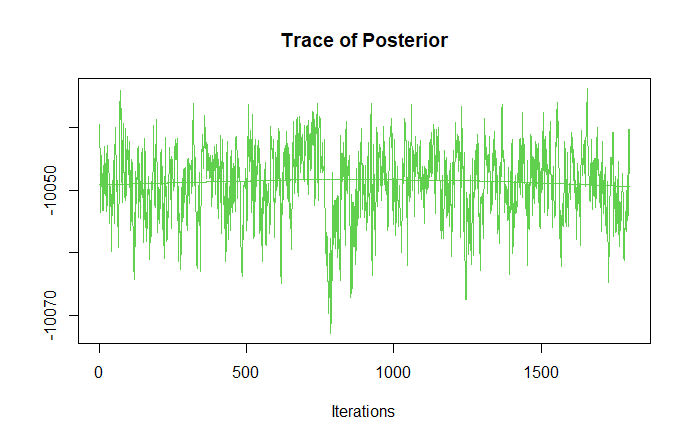
\includegraphics[width=1\linewidth]{img/Rplot} 

}

\caption{MCMC trace from the Cystopteridaceae `r homologizer` analysis}\label{fig:image4}
\end{figure}

\hypertarget{summarizing-and-visiualizing-traces-of-specific-parameter}{%
\subsection{Summarizing and Visiualizing Traces of specific parameter}\label{summarizing-and-visiualizing-traces-of-specific-parameter}}

In order to summarize the traces of specific parameters, \texttt{RevGadgets} uses the \texttt{SummarizeTrace()} function to calculate the mean and 95\% credible interval for quantitative and qualitative variables. in this study, we estimated a substitution rate multiplier for each of the alignments except the first one and drew the rate multipliers from an exponential distribution. To examine the rate\_multiplier parameter values in our trace file, we summarize their distributions using this code below:

\begin{Shaded}
\begin{Highlighting}[]
\FunctionTok{summarizeTrace}\NormalTok{(}\AttributeTok{trace =}\NormalTok{ trace\_quant, }\AttributeTok{vars =}  \FunctionTok{c}\NormalTok{(}\StringTok{"rate\_multiplier[2]"}\NormalTok{,}\StringTok{"rate\_multiplier[3]"}\NormalTok{,}\StringTok{"rate\_multiplier[4]"}\NormalTok{))}
\end{Highlighting}
\end{Shaded}

\begin{verbatim}
## $`rate_multiplier[2]`
## $`rate_multiplier[2]`$trace_1
##          mean        median           MAP  quantile_2.5 quantile_97.5 
##      1.601059      1.596110      1.617082      1.308977      1.972417 
## 
## 
## $`rate_multiplier[3]`
## $`rate_multiplier[3]`$trace_1
##          mean        median           MAP  quantile_2.5 quantile_97.5 
##     0.7831243     0.7744505     0.7579131     0.6115875     0.9833560 
## 
## 
## $`rate_multiplier[4]`
## $`rate_multiplier[4]`$trace_1
##          mean        median           MAP  quantile_2.5 quantile_97.5 
##      1.239250      1.237225      1.232346      1.017644      1.488608
\end{verbatim}

Then to plot these distributions. \texttt{plotTrace()} produces a list of ggplot2 objects, with multiple plots of multiple runs in the trace object.

\begin{Shaded}
\begin{Highlighting}[]
\FunctionTok{plotTrace}\NormalTok{(}\AttributeTok{trace =}\NormalTok{ trace\_quant, }\AttributeTok{vars =} \FunctionTok{c}\NormalTok{(}\StringTok{"rate\_multiplier[2]"}\NormalTok{,}\StringTok{"rate\_multiplier[3]"}\NormalTok{,}\StringTok{"rate\_multiplier[4]"}\NormalTok{))[[}\DecValTok{1}\NormalTok{]]}
\end{Highlighting}
\end{Shaded}

\begin{verbatim}
## Using  as id variables
\end{verbatim}

\textbackslash begin\{figure\}

\{\centering 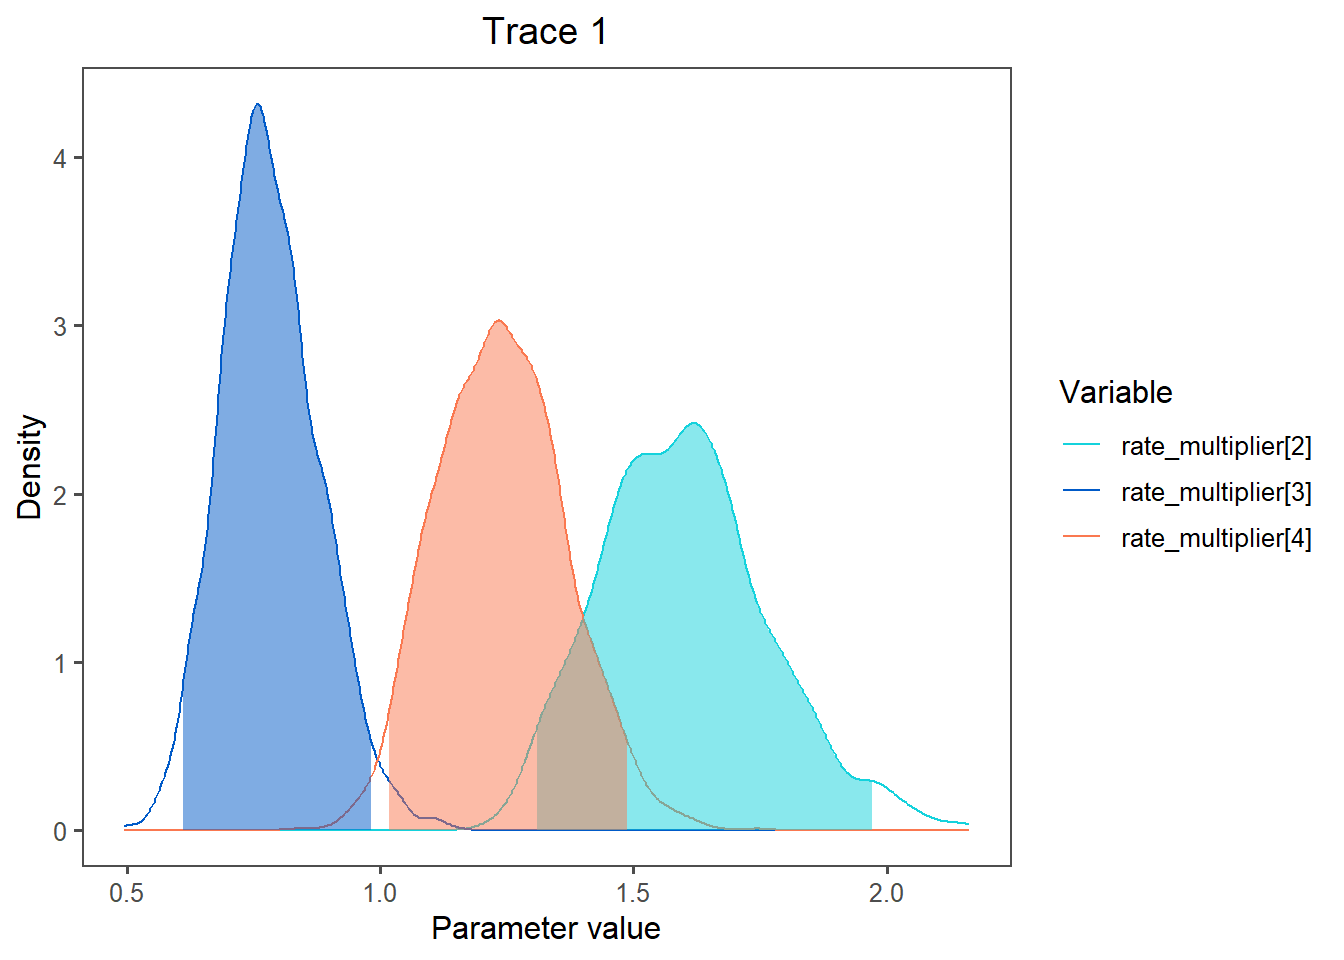
\includegraphics[width=1\linewidth]{_main_files/figure-latex/image6-1}

\}

\textbackslash caption\{The posterior densities of the nucleotide rate multipliers under a GTR substitution model. Colored areas under the curve correspond to the 95\% credible interval.\}\label{fig:image6}
\textbackslash end\{figure\}

\hypertarget{summarizing-homologizer-phasing-estimates-and-plotting-it-in-r}{%
\subsection{\texorpdfstring{Summarizing \texttt{homologizer} Phasing Estimates and Plotting it in R}{Summarizing homologizer Phasing Estimates and Plotting it in R}}\label{summarizing-homologizer-phasing-estimates-and-plotting-it-in-r}}

\texttt{homologizer} analysis ends with the creation of a tree file \texttt{homologizer\_output/homologizer\_map.tree} that can be plotted and rooted in software like \href{http://tree.bio.ed.ac.uk/software/figtree/}{FigTree} or \href{https://cran.r-project.org/web/packages/ape/index.html}{APE}. However, these software can't be used to properly summarize the phasing estimates of \texttt{homologizer} analysis. R can be used to achieve this task. The piece of R code below summarizes and plots the phasing estimates of \texttt{homologizer} analysis. This code can be found \href{https://github.com/Chinedum335/Semester_Project/tree/main/5_Code}{here}

\begin{Shaded}
\begin{Highlighting}[]
\NormalTok{genecopyFn}\OtherTok{=}\StringTok{\textquotesingle{}../1\_Raw\_Data/cystopteridaceae\_genomes.csv\textquotesingle{}}
\NormalTok{tree\_file }\OtherTok{=} \StringTok{\textquotesingle{}../4\_Output\_Trees/homologizer\_output/homologizer\_map\_rooted.trees\textquotesingle{}}
\NormalTok{input\_dir }\OtherTok{=} \StringTok{\textquotesingle{}../4\_Output\_Trees/homologizer\_output/\textquotesingle{}}
\NormalTok{output\_dir }\OtherTok{=} \StringTok{\textquotesingle{}../4\_Output\_Trees/homologizer\_output/\textquotesingle{}}
\NormalTok{prefix }\OtherTok{=} \StringTok{\textquotesingle{}../4\_Output\_Trees/homologizer\_output/homologizer\textquotesingle{}}


\CommentTok{\# Required packages}

\CommentTok{\#library(ggplot2)}
\CommentTok{\#library(plyr)}
\CommentTok{\#library(magrittr)}
\CommentTok{\#library(tidyr)}
\CommentTok{\#library(dplyr)}
\CommentTok{\#library(ggtree)}
\CommentTok{\#library(ape)}


\NormalTok{genecopymap }\OtherTok{=} \FunctionTok{read.csv}\NormalTok{(genecopyFn,}\AttributeTok{header=}\NormalTok{T,}\AttributeTok{stringsAsFactors=}\ConstantTok{TRUE}\NormalTok{)}
\NormalTok{samples }\OtherTok{=} \FunctionTok{split}\NormalTok{(genecopymap}\SpecialCharTok{$}\NormalTok{Subgenome,genecopymap}\SpecialCharTok{$}\NormalTok{Sample)}

\CommentTok{\# names of the loci in the log file}
\NormalTok{loci }\OtherTok{=} \FunctionTok{names}\NormalTok{(genecopymap)[}\DecValTok{3}\SpecialCharTok{:}\FunctionTok{length}\NormalTok{(genecopymap)]}

\CommentTok{\# what percentage of MCMC samples to exclude?}
\NormalTok{burnin }\OtherTok{=} \FloatTok{0.1}

\CommentTok{\# modified from ggtree gheatmap}
\NormalTok{homologized }\OtherTok{=} \ControlFlowTok{function}\NormalTok{ (p, data, data\_labels, }\AttributeTok{offset =} \DecValTok{0}\NormalTok{, }\AttributeTok{width =} \DecValTok{1}\NormalTok{, }\AttributeTok{low =} \StringTok{"green"}\NormalTok{, mid, }\AttributeTok{high =} \StringTok{"red"}\NormalTok{,}
                        \AttributeTok{color =} \StringTok{"white"}\NormalTok{, }\AttributeTok{colnames =} \ConstantTok{TRUE}\NormalTok{, }\AttributeTok{colnames\_position =} \StringTok{"bottom"}\NormalTok{,}
                        \AttributeTok{colnames\_angle =} \DecValTok{0}\NormalTok{, }\AttributeTok{colnames\_level =} \ConstantTok{NULL}\NormalTok{, }\AttributeTok{colnames\_offset\_x =} \DecValTok{0}\NormalTok{,}
                        \AttributeTok{colnames\_offset\_y =} \DecValTok{0}\NormalTok{, }\AttributeTok{font.size =} \DecValTok{4}\NormalTok{, }\AttributeTok{family =} \StringTok{""}\NormalTok{, }\AttributeTok{hjust =} \FloatTok{0.5}\NormalTok{,}
                        \AttributeTok{legend\_title =} \StringTok{"value"}\NormalTok{)}
\NormalTok{\{}
\NormalTok{  colnames\_position }\SpecialCharTok{\%\textless{}\textgreater{}\%} \FunctionTok{match.arg}\NormalTok{(}\FunctionTok{c}\NormalTok{(}\StringTok{"bottom"}\NormalTok{, }\StringTok{"top"}\NormalTok{))}
\NormalTok{  variable }\OtherTok{\textless{}{-}}\NormalTok{ value }\OtherTok{\textless{}{-}}\NormalTok{ lab }\OtherTok{\textless{}{-}}\NormalTok{ y }\OtherTok{\textless{}{-}} \ConstantTok{NULL}
\NormalTok{  width }\OtherTok{\textless{}{-}}\NormalTok{ width }\SpecialCharTok{*}\NormalTok{ (p}\SpecialCharTok{$}\NormalTok{data}\SpecialCharTok{$}\NormalTok{x }\SpecialCharTok{\%\textgreater{}\%} \FunctionTok{range}\NormalTok{(}\AttributeTok{na.rm =} \ConstantTok{TRUE}\NormalTok{) }\SpecialCharTok{\%\textgreater{}\%}\NormalTok{ diff)}\SpecialCharTok{/}\FunctionTok{ncol}\NormalTok{(data)}
\NormalTok{  isTip }\OtherTok{\textless{}{-}}\NormalTok{ x }\OtherTok{\textless{}{-}}\NormalTok{ y }\OtherTok{\textless{}{-}}\NormalTok{ variable }\OtherTok{\textless{}{-}}\NormalTok{ value }\OtherTok{\textless{}{-}}\NormalTok{ from }\OtherTok{\textless{}{-}}\NormalTok{ to }\OtherTok{\textless{}{-}} \ConstantTok{NULL}
\NormalTok{  df }\OtherTok{\textless{}{-}}\NormalTok{ p}\SpecialCharTok{$}\NormalTok{data}
\NormalTok{  nodeCo }\OtherTok{\textless{}{-}} \FunctionTok{intersect}\NormalTok{(df }\SpecialCharTok{\%\textgreater{}\%} \FunctionTok{filter}\NormalTok{(}\FunctionTok{is.na}\NormalTok{(x)) }\SpecialCharTok{\%\textgreater{}\%} \FunctionTok{select}\NormalTok{(.data}\SpecialCharTok{$}\NormalTok{parent,}
\NormalTok{                                                         .data}\SpecialCharTok{$}\NormalTok{node) }\SpecialCharTok{\%\textgreater{}\%} \FunctionTok{unlist}\NormalTok{(), df }\SpecialCharTok{\%\textgreater{}\%} \FunctionTok{filter}\NormalTok{(}\SpecialCharTok{!}\FunctionTok{is.na}\NormalTok{(x)) }\SpecialCharTok{\%\textgreater{}\%}
                        \FunctionTok{select}\NormalTok{(.data}\SpecialCharTok{$}\NormalTok{parent, .data}\SpecialCharTok{$}\NormalTok{node) }\SpecialCharTok{\%\textgreater{}\%} \FunctionTok{unlist}\NormalTok{())}
\NormalTok{  labCo }\OtherTok{\textless{}{-}}\NormalTok{ df }\SpecialCharTok{\%\textgreater{}\%} \FunctionTok{filter}\NormalTok{(.data}\SpecialCharTok{$}\NormalTok{node }\SpecialCharTok{\%in\%}\NormalTok{ nodeCo) }\SpecialCharTok{\%\textgreater{}\%} \FunctionTok{select}\NormalTok{(.data}\SpecialCharTok{$}\NormalTok{label) }\SpecialCharTok{\%\textgreater{}\%}
    \FunctionTok{unlist}\NormalTok{()}
\NormalTok{  selCo }\OtherTok{\textless{}{-}} \FunctionTok{intersect}\NormalTok{(labCo, }\FunctionTok{rownames}\NormalTok{(data))}
\NormalTok{  isSel }\OtherTok{\textless{}{-}}\NormalTok{ df}\SpecialCharTok{$}\NormalTok{label }\SpecialCharTok{\%in\%}\NormalTok{ selCo}
\NormalTok{  df }\OtherTok{\textless{}{-}}\NormalTok{ df[df}\SpecialCharTok{$}\NormalTok{isTip }\SpecialCharTok{|}\NormalTok{ isSel, ]}
\NormalTok{  start }\OtherTok{\textless{}{-}} \FunctionTok{max}\NormalTok{(df}\SpecialCharTok{$}\NormalTok{x, }\AttributeTok{na.rm =} \ConstantTok{TRUE}\NormalTok{) }\SpecialCharTok{+}\NormalTok{ offset}
\NormalTok{  dd }\OtherTok{\textless{}{-}} \FunctionTok{as.data.frame}\NormalTok{(data)}
\NormalTok{  dd2 }\OtherTok{\textless{}{-}} \FunctionTok{as.data.frame}\NormalTok{(data\_labels)}
\NormalTok{  i }\OtherTok{\textless{}{-}} \FunctionTok{order}\NormalTok{(df}\SpecialCharTok{$}\NormalTok{y)}
\NormalTok{  i }\OtherTok{\textless{}{-}}\NormalTok{ i[}\SpecialCharTok{!}\FunctionTok{is.na}\NormalTok{(df}\SpecialCharTok{$}\NormalTok{y[i])]}
\NormalTok{  lab }\OtherTok{\textless{}{-}}\NormalTok{ df}\SpecialCharTok{$}\NormalTok{label[i]}
\NormalTok{  dd }\OtherTok{\textless{}{-}}\NormalTok{ dd[}\FunctionTok{match}\NormalTok{(lab, }\FunctionTok{rownames}\NormalTok{(dd)), , drop }\OtherTok{=} \ConstantTok{FALSE}\NormalTok{]}
\NormalTok{  dd2 }\OtherTok{\textless{}{-}}\NormalTok{ dd2[}\FunctionTok{match}\NormalTok{(lab, }\FunctionTok{rownames}\NormalTok{(dd2)), , drop }\OtherTok{=} \ConstantTok{FALSE}\NormalTok{]}
\NormalTok{  dd}\SpecialCharTok{$}\NormalTok{y }\OtherTok{\textless{}{-}} \FunctionTok{sort}\NormalTok{(df}\SpecialCharTok{$}\NormalTok{y)}
\NormalTok{  dd2}\SpecialCharTok{$}\NormalTok{y }\OtherTok{\textless{}{-}} \FunctionTok{sort}\NormalTok{(df}\SpecialCharTok{$}\NormalTok{y)}
\NormalTok{  dd}\SpecialCharTok{$}\NormalTok{lab }\OtherTok{\textless{}{-}}\NormalTok{ lab}
\NormalTok{  dd2}\SpecialCharTok{$}\NormalTok{lab }\OtherTok{\textless{}{-}}\NormalTok{ lab}
\NormalTok{  dd }\OtherTok{\textless{}{-}} \FunctionTok{gather}\NormalTok{(dd, variable, value, }\SpecialCharTok{{-}}\FunctionTok{c}\NormalTok{(lab, y))}
\NormalTok{  dd2 }\OtherTok{\textless{}{-}} \FunctionTok{gather}\NormalTok{(dd2, variable, value, }\SpecialCharTok{{-}}\FunctionTok{c}\NormalTok{(lab, y))}
\NormalTok{  i }\OtherTok{\textless{}{-}} \FunctionTok{which}\NormalTok{(dd}\SpecialCharTok{$}\NormalTok{value }\SpecialCharTok{==} \StringTok{""}\NormalTok{)}
  \ControlFlowTok{if}\NormalTok{ (}\FunctionTok{length}\NormalTok{(i) }\SpecialCharTok{\textgreater{}} \DecValTok{0}\NormalTok{) \{}
\NormalTok{    dd}\SpecialCharTok{$}\NormalTok{value[i] }\OtherTok{\textless{}{-}} \ConstantTok{NA}
\NormalTok{    dd2}\SpecialCharTok{$}\NormalTok{value[i] }\OtherTok{\textless{}{-}} \ConstantTok{NA}
\NormalTok{  \}}
  \ControlFlowTok{if}\NormalTok{ (}\FunctionTok{is.null}\NormalTok{(colnames\_level)) \{}
\NormalTok{    dd}\SpecialCharTok{$}\NormalTok{variable }\OtherTok{\textless{}{-}} \FunctionTok{factor}\NormalTok{(dd}\SpecialCharTok{$}\NormalTok{variable, }\AttributeTok{levels =} \FunctionTok{colnames}\NormalTok{(data))}
\NormalTok{  \}}
  \ControlFlowTok{else}\NormalTok{ \{}
\NormalTok{    dd}\SpecialCharTok{$}\NormalTok{variable }\OtherTok{\textless{}{-}} \FunctionTok{factor}\NormalTok{(dd}\SpecialCharTok{$}\NormalTok{variable, }\AttributeTok{levels =}\NormalTok{ colnames\_level)}
\NormalTok{  \}}
\NormalTok{  V2 }\OtherTok{\textless{}{-}}\NormalTok{ start }\SpecialCharTok{+} \FunctionTok{as.numeric}\NormalTok{(dd}\SpecialCharTok{$}\NormalTok{variable) }\SpecialCharTok{*}\NormalTok{ width}
\NormalTok{  mapping }\OtherTok{\textless{}{-}} \FunctionTok{data.frame}\NormalTok{(}\AttributeTok{from =}\NormalTok{ dd}\SpecialCharTok{$}\NormalTok{variable, }\AttributeTok{to =}\NormalTok{ V2)}
\NormalTok{  mapping }\OtherTok{\textless{}{-}} \FunctionTok{unique}\NormalTok{(mapping)}
\NormalTok{  dd}\SpecialCharTok{$}\NormalTok{x }\OtherTok{\textless{}{-}}\NormalTok{ V2}
\NormalTok{  dd2}\SpecialCharTok{$}\NormalTok{x }\OtherTok{\textless{}{-}}\NormalTok{ V2}
\NormalTok{  dd}\SpecialCharTok{$}\NormalTok{width }\OtherTok{\textless{}{-}}\NormalTok{ width}
\NormalTok{  dd2}\SpecialCharTok{$}\NormalTok{width }\OtherTok{\textless{}{-}}\NormalTok{ width}
\NormalTok{  dd[[}\StringTok{".panel"}\NormalTok{]] }\OtherTok{\textless{}{-}} \FunctionTok{factor}\NormalTok{(}\StringTok{"Tree"}\NormalTok{)}
\NormalTok{  dd2[[}\StringTok{".panel"}\NormalTok{]] }\OtherTok{\textless{}{-}} \FunctionTok{factor}\NormalTok{(}\StringTok{"Tree"}\NormalTok{)}
  \ControlFlowTok{if}\NormalTok{ (}\FunctionTok{is.null}\NormalTok{(color)) \{}
\NormalTok{    p2 }\OtherTok{\textless{}{-}}\NormalTok{ p }\SpecialCharTok{+} \FunctionTok{geom\_tile}\NormalTok{(}\AttributeTok{data =}\NormalTok{ dd, }\FunctionTok{aes}\NormalTok{(x, y, }\AttributeTok{fill =}\NormalTok{ value),}
                        \AttributeTok{width =}\NormalTok{ width, }\AttributeTok{inherit.aes =} \ConstantTok{FALSE}\NormalTok{)}
\NormalTok{  \}}
  \ControlFlowTok{else}\NormalTok{ \{}
\NormalTok{    p2 }\OtherTok{\textless{}{-}}\NormalTok{ p }\SpecialCharTok{+} \FunctionTok{geom\_tile}\NormalTok{(}\AttributeTok{data =}\NormalTok{ dd, }\FunctionTok{aes}\NormalTok{(x, y, }\AttributeTok{fill =}\NormalTok{ value),}
                        \AttributeTok{width =}\NormalTok{ width, }\AttributeTok{color =}\NormalTok{ color, }\AttributeTok{inherit.aes =} \ConstantTok{FALSE}\NormalTok{)}
\NormalTok{    p2 }\OtherTok{\textless{}{-}}\NormalTok{ p2 }\SpecialCharTok{+} \FunctionTok{geom\_text}\NormalTok{(}\AttributeTok{data =}\NormalTok{ dd2, }\FunctionTok{aes}\NormalTok{(x, y, }\AttributeTok{label=}\NormalTok{value), }\AttributeTok{size=}\DecValTok{1}\NormalTok{, }\AttributeTok{inherit.aes =} \ConstantTok{FALSE}\NormalTok{)}
    
    \CommentTok{\# }\AlertTok{TODO}
    \CommentTok{\#print(dd)}
\NormalTok{    dd3 }\OtherTok{=} \FunctionTok{data.frame}\NormalTok{()}
\NormalTok{    start\_x }\OtherTok{=} \FunctionTok{max}\NormalTok{(dd}\SpecialCharTok{$}\NormalTok{x)}
\NormalTok{    height }\OtherTok{=} \FunctionTok{max}\NormalTok{(dd}\SpecialCharTok{$}\NormalTok{y)}
\NormalTok{    margin }\OtherTok{=} \FloatTok{0.006}
    \ControlFlowTok{for}\NormalTok{ (y }\ControlFlowTok{in} \FunctionTok{unique}\NormalTok{(dd}\SpecialCharTok{$}\NormalTok{y)) \{}
\NormalTok{      pp }\OtherTok{=} \FunctionTok{mean}\NormalTok{(dd[dd}\SpecialCharTok{$}\NormalTok{y }\SpecialCharTok{==}\NormalTok{ y, }\StringTok{\textquotesingle{}value\textquotesingle{}}\NormalTok{], }\AttributeTok{na.rm=}\ConstantTok{TRUE}\NormalTok{)}
\NormalTok{      dd4 }\OtherTok{=} \FunctionTok{data.frame}\NormalTok{(}\AttributeTok{pp =}\NormalTok{ pp, }\AttributeTok{x =}\NormalTok{ pp}\SpecialCharTok{/}\DecValTok{200} \SpecialCharTok{+}\NormalTok{ margin }\SpecialCharTok{+}\NormalTok{ start\_x, }\AttributeTok{y=}\NormalTok{y)}
\NormalTok{      dd3 }\OtherTok{=} \FunctionTok{rbind}\NormalTok{(dd3, dd4)}
\NormalTok{    \}}
    \CommentTok{\#print(dd3)}
\NormalTok{    p2 }\OtherTok{\textless{}{-}}\NormalTok{ p2 }\SpecialCharTok{+} \FunctionTok{geom\_segment}\NormalTok{(}\FunctionTok{aes}\NormalTok{(}\AttributeTok{x=}\NormalTok{start\_x}\SpecialCharTok{+}\NormalTok{margin, }\AttributeTok{xend=}\DecValTok{1}\SpecialCharTok{/}\DecValTok{200} \SpecialCharTok{+}\NormalTok{ start\_x }\SpecialCharTok{+}\NormalTok{ margin, }\AttributeTok{y=}\FloatTok{0.2}\NormalTok{, }\AttributeTok{yend=}\FloatTok{0.2}\NormalTok{), }\AttributeTok{size=}\FloatTok{0.5}\NormalTok{, }\AttributeTok{inherit.aes =} \ConstantTok{FALSE}\NormalTok{)}
\NormalTok{    p2 }\OtherTok{\textless{}{-}}\NormalTok{ p2 }\SpecialCharTok{+} \FunctionTok{geom\_segment}\NormalTok{(}\FunctionTok{aes}\NormalTok{(}\AttributeTok{x=}\DecValTok{1}\SpecialCharTok{/}\DecValTok{200}\SpecialCharTok{+}\NormalTok{start\_x}\SpecialCharTok{+}\NormalTok{margin, }\AttributeTok{xend=}\DecValTok{1}\SpecialCharTok{/}\DecValTok{200}\SpecialCharTok{+}\NormalTok{start\_x}\SpecialCharTok{+}\NormalTok{margin, }\AttributeTok{y=}\FloatTok{0.5}\NormalTok{, }\AttributeTok{yend=}\NormalTok{height), }\AttributeTok{color=}\StringTok{\textquotesingle{}grey85\textquotesingle{}}\NormalTok{, }\AttributeTok{linetype=}\StringTok{\textquotesingle{}dotted\textquotesingle{}}\NormalTok{, }\AttributeTok{size=}\FloatTok{0.35}\NormalTok{, }\AttributeTok{inherit.aes =} \ConstantTok{FALSE}\NormalTok{)}
\NormalTok{    p2 }\OtherTok{\textless{}{-}}\NormalTok{ p2 }\SpecialCharTok{+} \FunctionTok{geom\_segment}\NormalTok{(}\FunctionTok{aes}\NormalTok{(}\AttributeTok{x=}\NormalTok{start\_x}\SpecialCharTok{+}\NormalTok{margin, }\AttributeTok{xend=}\NormalTok{start\_x}\SpecialCharTok{+}\NormalTok{margin, }\AttributeTok{y=}\FloatTok{0.5}\NormalTok{, }\AttributeTok{yend=}\NormalTok{height), }\AttributeTok{color=}\StringTok{\textquotesingle{}grey85\textquotesingle{}}\NormalTok{, }\AttributeTok{linetype=}\StringTok{\textquotesingle{}dotted\textquotesingle{}}\NormalTok{, }\AttributeTok{size=}\FloatTok{0.35}\NormalTok{, }\AttributeTok{inherit.aes =} \ConstantTok{FALSE}\NormalTok{)}
\NormalTok{    p2 }\OtherTok{\textless{}{-}}\NormalTok{ p2 }\SpecialCharTok{+} \FunctionTok{geom\_point}\NormalTok{(}\AttributeTok{data =}\NormalTok{ dd3, }\FunctionTok{aes}\NormalTok{(x, y, }\AttributeTok{color=}\NormalTok{pp), }\AttributeTok{size=}\FloatTok{1.25}\NormalTok{, }\AttributeTok{inherit.aes =} \ConstantTok{FALSE}\NormalTok{, }\AttributeTok{show.legend=}\ConstantTok{FALSE}\NormalTok{)}
\NormalTok{    p2 }\OtherTok{\textless{}{-}}\NormalTok{ p2 }\SpecialCharTok{+} \FunctionTok{geom\_text}\NormalTok{(}\AttributeTok{label=}\StringTok{\textquotesingle{}0.0\textquotesingle{}}\NormalTok{, }\AttributeTok{x=}\NormalTok{start\_x}\SpecialCharTok{+}\NormalTok{margin, }\AttributeTok{y=}\SpecialCharTok{{-}}\FloatTok{0.2}\NormalTok{, }\AttributeTok{size=}\FloatTok{1.25}\NormalTok{, }\AttributeTok{color=}\StringTok{\textquotesingle{}grey50\textquotesingle{}}\NormalTok{)}
\NormalTok{    p2 }\OtherTok{\textless{}{-}}\NormalTok{ p2 }\SpecialCharTok{+} \FunctionTok{geom\_text}\NormalTok{(}\AttributeTok{label=}\StringTok{\textquotesingle{}1.0\textquotesingle{}}\NormalTok{, }\AttributeTok{x=}\NormalTok{start\_x}\SpecialCharTok{+}\NormalTok{margin}\SpecialCharTok{+}\DecValTok{1}\SpecialCharTok{/}\DecValTok{200}\NormalTok{, }\AttributeTok{y=}\SpecialCharTok{{-}}\FloatTok{0.2}\NormalTok{, }\AttributeTok{size=}\FloatTok{1.25}\NormalTok{, }\AttributeTok{color=}\StringTok{\textquotesingle{}grey50\textquotesingle{}}\NormalTok{)}
\NormalTok{  \}}
  \ControlFlowTok{if}\NormalTok{ (methods}\SpecialCharTok{::}\FunctionTok{is}\NormalTok{(dd}\SpecialCharTok{$}\NormalTok{value, }\StringTok{"numeric"}\NormalTok{)) \{}
\NormalTok{    midpoint }\OtherTok{=} \FunctionTok{max}\NormalTok{(dd}\SpecialCharTok{$}\NormalTok{value, }\AttributeTok{na.rm=}\ConstantTok{TRUE}\NormalTok{) }\SpecialCharTok{{-}} \FunctionTok{min}\NormalTok{(dd}\SpecialCharTok{$}\NormalTok{value, }\AttributeTok{na.rm=}\ConstantTok{TRUE}\NormalTok{)}
\NormalTok{    midpoint }\OtherTok{=}\NormalTok{ midpoint}\SpecialCharTok{/}\DecValTok{2} \SpecialCharTok{+} \FunctionTok{min}\NormalTok{(dd}\SpecialCharTok{$}\NormalTok{value, }\AttributeTok{na.rm=}\ConstantTok{TRUE}\NormalTok{) }
\NormalTok{    midpoint }\OtherTok{=} \FloatTok{0.25}
\NormalTok{    p2 }\OtherTok{\textless{}{-}}\NormalTok{ p2 }\SpecialCharTok{+} \FunctionTok{scale\_fill\_gradient2}\NormalTok{(}\AttributeTok{low =}\NormalTok{ low, }\AttributeTok{mid=}\NormalTok{mid, }\AttributeTok{high =}\NormalTok{ high, }\AttributeTok{midpoint=}\NormalTok{midpoint,}
                                    \AttributeTok{na.value =} \StringTok{"white"}\NormalTok{, }\AttributeTok{name =}\NormalTok{ legend\_title, }\AttributeTok{limits=}\FunctionTok{c}\NormalTok{(}\DecValTok{0}\NormalTok{,}\DecValTok{1}\NormalTok{))}
\NormalTok{    p2 }\OtherTok{\textless{}{-}}\NormalTok{ p2 }\SpecialCharTok{+} \FunctionTok{scale\_color\_gradient2}\NormalTok{(}\AttributeTok{low =}\NormalTok{ low, }\AttributeTok{mid=}\NormalTok{mid, }\AttributeTok{high =}\NormalTok{ high, }\AttributeTok{midpoint=}\NormalTok{midpoint,}
                                     \AttributeTok{na.value =} \StringTok{"white"}\NormalTok{, }\AttributeTok{name =}\NormalTok{ legend\_title, }\AttributeTok{limits=}\FunctionTok{c}\NormalTok{(}\DecValTok{0}\NormalTok{,}\DecValTok{1}\NormalTok{))}
    \CommentTok{\#na.value = NA, name = legend\_title)}
\NormalTok{  \}}
  \ControlFlowTok{else}\NormalTok{ \{}
\NormalTok{    p2 }\OtherTok{\textless{}{-}}\NormalTok{ p2 }\SpecialCharTok{+} \FunctionTok{scale\_fill\_discrete}\NormalTok{(}\AttributeTok{na.value =} \ConstantTok{NA}\NormalTok{, }\AttributeTok{name =}\NormalTok{ legend\_title)}
\NormalTok{  \}}
  \ControlFlowTok{if}\NormalTok{ (colnames) \{}
    \ControlFlowTok{if}\NormalTok{ (colnames\_position }\SpecialCharTok{==} \StringTok{"bottom"}\NormalTok{) \{}
\NormalTok{      y }\OtherTok{\textless{}{-}} \DecValTok{0}
\NormalTok{    \}}
    \ControlFlowTok{else}\NormalTok{ \{}
\NormalTok{      y }\OtherTok{\textless{}{-}} \FunctionTok{max}\NormalTok{(p}\SpecialCharTok{$}\NormalTok{data}\SpecialCharTok{$}\NormalTok{y) }\SpecialCharTok{+} \DecValTok{1}
\NormalTok{    \}}
\NormalTok{    mapping}\SpecialCharTok{$}\NormalTok{y }\OtherTok{\textless{}{-}}\NormalTok{ y}
\NormalTok{    mapping[[}\StringTok{".panel"}\NormalTok{]] }\OtherTok{\textless{}{-}} \FunctionTok{factor}\NormalTok{(}\StringTok{"Tree"}\NormalTok{)}
\NormalTok{    p2 }\OtherTok{\textless{}{-}}\NormalTok{ p2 }\SpecialCharTok{+} \FunctionTok{geom\_text}\NormalTok{(}\AttributeTok{data =}\NormalTok{ mapping, }\FunctionTok{aes}\NormalTok{(}\AttributeTok{x =}\NormalTok{ to, }\AttributeTok{y =}\NormalTok{ y,}
                                             \AttributeTok{label =}\NormalTok{ from), }\AttributeTok{size =}\NormalTok{ font.size, }\AttributeTok{family =}\NormalTok{ family,}
                         \AttributeTok{inherit.aes =} \ConstantTok{FALSE}\NormalTok{, }\AttributeTok{angle =}\NormalTok{ colnames\_angle, }\AttributeTok{nudge\_x =}\NormalTok{ colnames\_offset\_x,}
                         \AttributeTok{nudge\_y =}\NormalTok{ colnames\_offset\_y, }\AttributeTok{hjust =}\NormalTok{ hjust)}
\NormalTok{  \}}
\NormalTok{  p2 }\OtherTok{\textless{}{-}}\NormalTok{ p2 }\SpecialCharTok{+} \FunctionTok{theme}\NormalTok{(}\AttributeTok{legend.position =} \StringTok{"right"}\NormalTok{)}
  \ControlFlowTok{if}\NormalTok{ (}\SpecialCharTok{!}\NormalTok{colnames) \{}
\NormalTok{    p2 }\OtherTok{\textless{}{-}}\NormalTok{ p2 }\SpecialCharTok{+} \FunctionTok{scale\_y\_continuous}\NormalTok{(}\AttributeTok{expand =} \FunctionTok{c}\NormalTok{(}\DecValTok{0}\NormalTok{, }\DecValTok{0}\NormalTok{))}
\NormalTok{  \}}
  \FunctionTok{attr}\NormalTok{(p2, }\StringTok{"mapping"}\NormalTok{) }\OtherTok{\textless{}{-}}\NormalTok{ mapping}
  \FunctionTok{return}\NormalTok{(p2)}
\NormalTok{\}}



\CommentTok{\# polyploid samples and their tips}
\CommentTok{\# samples = list(\textquotesingle{}A\_taiwaniana\_6137\textquotesingle{} = c("A\_taiwaniana\_6137\_A", "A\_taiwaniana\_6137\_B"),}
\CommentTok{\#                \textquotesingle{}A\_tenuisecta\_sp2\_8704\textquotesingle{} = c("A\_tenuisecta\_sp2\_8704\_A", "A\_tenuisecta\_sp2\_8704\_B"),}
\CommentTok{\#                \textquotesingle{}A\_tenuisecta\_sp3\_8745\textquotesingle{} = c("A\_tenuisecta\_sp3\_8745\_A", "A\_tenuisecta\_sp3\_8745\_B"),}
\CommentTok{\#                \textquotesingle{}C\_diaphana\_6380\textquotesingle{} = c("C\_diaphana\_6380\_A", "C\_diaphana\_6380\_B"),}
\CommentTok{\#                \textquotesingle{}C\_fragilis\_sp1\_7009\textquotesingle{} = c("C\_fragilis\_sp1\_7009\_A", "C\_fragilis\_sp1\_7009\_B"),}
\CommentTok{\#                \textquotesingle{}C\_fragilis\_sp2\_7248\textquotesingle{} = c("C\_fragilis\_sp2\_7248\_A", "C\_fragilis\_sp2\_7248\_B"),}
\CommentTok{\#                \textquotesingle{}C\_montana\_7943\textquotesingle{} = c("C\_montana\_7943\_A", "C\_montana\_7943\_B"),}
\CommentTok{\#                \textquotesingle{}C\_pellucida\_6055\textquotesingle{}  = c("C\_pellucida\_6055\_A", "C\_pellucida\_6055\_B"),}
\CommentTok{\#                \textquotesingle{}C\_sudetica\_8674\textquotesingle{} = c("C\_sudetica\_8674\_A", "C\_sudetica\_8674\_B"),}
\CommentTok{\#                \textquotesingle{}C\_tasmanica\_6379\textquotesingle{} = c("C\_tasmanica\_6379\_A", "C\_tasmanica\_6379\_B"),}
\CommentTok{\#                \textquotesingle{}C\_tenuis\_6387\textquotesingle{} = c("C\_tenuis\_6387\_A", "C\_tenuis\_6387\_B"),}
\CommentTok{\#                \textquotesingle{}C\_utahensis\_6848\textquotesingle{} = c("C\_utahensis\_6848\_A", "C\_utahensis\_6848\_B"),}
\CommentTok{\#                \textquotesingle{}G\_continentale\_6979\textquotesingle{} = c("G\_continentale\_6979\_A", "G\_continentale\_6979\_B"),}
\CommentTok{\#                \textquotesingle{}G\_disjunctum\_7751\textquotesingle{} = c("G\_disjunctum\_7751\_A", "G\_disjunctum\_7751\_B"),}
\CommentTok{\#                \textquotesingle{}G\_oyamense\_sp2\_8739\textquotesingle{} = c("G\_oyamense\_sp2\_8739\_A", "G\_oyamense\_sp2\_8739\_B"),}
\CommentTok{\#                \textquotesingle{}G\_remotepinnatum\_4862\textquotesingle{} = c("G\_remotepinnatum\_4862\_A", "G\_remotepinnatum\_4862\_B"),}
\CommentTok{\#                \textquotesingle{}G\_robertianum\_7945\textquotesingle{} = c("G\_robertianum\_7945\_A", "G\_robertianum\_7945\_B"),}
\CommentTok{\#                \textquotesingle{}G\_dryopteris\_7981\textquotesingle{} = c("G\_dryopteris\_7981\_A", "G\_dryopteris\_7981\_B", "G\_dryopteris\_7981\_C", "G\_dryopteris\_7981\_D"),}
\CommentTok{\#                \textquotesingle{}xCystocarpium\_7974\textquotesingle{} = c("xCystocarpium\_7974\_A", "xCystocarpium\_7974\_B", "xCystocarpium\_7974\_C","xCystocarpium\_7974\_D"))}


\CommentTok{\# populate empty dataframes to hold results}
\NormalTok{map\_prob\_results }\OtherTok{=} \FunctionTok{data.frame}\NormalTok{()}
\NormalTok{joint\_map\_phase\_results }\OtherTok{=} \FunctionTok{data.frame}\NormalTok{()}
\ControlFlowTok{for}\NormalTok{ (sample }\ControlFlowTok{in} \FunctionTok{names}\NormalTok{(samples)) \{}
\NormalTok{  sample\_joint\_map\_prob }\OtherTok{=} \FunctionTok{data.frame}\NormalTok{()}
\NormalTok{  sample\_joint\_map\_phase }\OtherTok{=} \FunctionTok{data.frame}\NormalTok{()}
  \ControlFlowTok{for}\NormalTok{ (i }\ControlFlowTok{in} \DecValTok{1}\SpecialCharTok{:}\FunctionTok{length}\NormalTok{(loci)) \{}
\NormalTok{    sample\_joint\_map\_prob[}\DecValTok{1}\NormalTok{, loci[i]] }\OtherTok{=} \FloatTok{0.0}
\NormalTok{    sample\_joint\_map\_phase[}\DecValTok{1}\NormalTok{, loci[i]] }\OtherTok{=} \StringTok{\textquotesingle{}\textquotesingle{}}
    \FunctionTok{row.names}\NormalTok{(sample\_joint\_map\_prob) }\OtherTok{=} \FunctionTok{c}\NormalTok{(sample)}
    \FunctionTok{row.names}\NormalTok{(sample\_joint\_map\_phase) }\OtherTok{=} \FunctionTok{c}\NormalTok{(sample)}
\NormalTok{  \}}
\NormalTok{  map\_prob\_results }\OtherTok{=} \FunctionTok{rbind}\NormalTok{(map\_prob\_results, sample\_joint\_map\_prob)}
\NormalTok{  joint\_map\_phase\_results }\OtherTok{=} \FunctionTok{rbind}\NormalTok{(joint\_map\_phase\_results, sample\_joint\_map\_phase)}
\NormalTok{\}}

\CommentTok{\# for each sample loop over each locus}
\NormalTok{marginal\_results }\OtherTok{=} \FunctionTok{data.frame}\NormalTok{()}
\ControlFlowTok{for}\NormalTok{ (sample }\ControlFlowTok{in} \FunctionTok{names}\NormalTok{(samples)) \{}

\NormalTok{  joint\_results }\OtherTok{=} \FunctionTok{data.frame}\NormalTok{()}
  \ControlFlowTok{for}\NormalTok{ (i }\ControlFlowTok{in} \DecValTok{1}\SpecialCharTok{:}\FunctionTok{length}\NormalTok{(loci)) \{}
    \CommentTok{\# read in file and exclude burnin}
\NormalTok{    f\_in }\OtherTok{=} \FunctionTok{paste0}\NormalTok{(prefix, }\StringTok{\textquotesingle{}\_locus\_\textquotesingle{}}\NormalTok{,i, }\StringTok{\textquotesingle{}\_phase.log\textquotesingle{}}\NormalTok{)}
\NormalTok{    d }\OtherTok{=} \FunctionTok{read.csv}\NormalTok{(f\_in, }\AttributeTok{sep=}\StringTok{\textquotesingle{}}\SpecialCharTok{\textbackslash{}t}\StringTok{\textquotesingle{}}\NormalTok{,}\AttributeTok{stringsAsFactors =} \ConstantTok{TRUE}\NormalTok{,}\AttributeTok{row.names=}\DecValTok{1}\NormalTok{)}
\NormalTok{    d }\OtherTok{=}\NormalTok{ d[}\FunctionTok{floor}\NormalTok{(}\FunctionTok{nrow}\NormalTok{(d)}\SpecialCharTok{*}\NormalTok{burnin)}\SpecialCharTok{:}\FunctionTok{nrow}\NormalTok{(d),]}
    
    \CommentTok{\# get joint phase assignments for this locus}
\NormalTok{    d1 }\OtherTok{=}\NormalTok{ d[, samples[[sample]]]}
\NormalTok{    joint\_results\_locus }\OtherTok{=} \FunctionTok{as.data.frame}\NormalTok{(}\FunctionTok{table}\NormalTok{(d1))}
\NormalTok{    joint\_results\_locus}\SpecialCharTok{$}\NormalTok{joint\_prob }\OtherTok{=}\NormalTok{ joint\_results\_locus}\SpecialCharTok{$}\NormalTok{Freq }\SpecialCharTok{/} \FunctionTok{sum}\NormalTok{(joint\_results\_locus}\SpecialCharTok{$}\NormalTok{Freq)}
\NormalTok{    joint\_results\_locus}\SpecialCharTok{$}\NormalTok{locus }\OtherTok{=}\NormalTok{ loci[i]}
\NormalTok{    joint\_results }\OtherTok{=} \FunctionTok{rbind}\NormalTok{(joint\_results, joint\_results\_locus) }
   
    \CommentTok{\# get the MAP joint phase for the plot}
\NormalTok{    map }\OtherTok{=} \FunctionTok{which}\NormalTok{(joint\_results\_locus[}\StringTok{\textquotesingle{}joint\_prob\textquotesingle{}}\NormalTok{] }\SpecialCharTok{==} \FunctionTok{max}\NormalTok{(joint\_results\_locus[}\StringTok{\textquotesingle{}joint\_prob\textquotesingle{}}\NormalTok{]))[}\DecValTok{1}\NormalTok{]}
    \ControlFlowTok{for}\NormalTok{ (tip }\ControlFlowTok{in}\NormalTok{ samples[[sample]]) \{}
      \CommentTok{\#map\_prob\_results[tip,loci[i]] = joint\_results\_locus[map, \textquotesingle{}joint\_prob\textquotesingle{}]}
\NormalTok{      joint\_map\_phase\_results[tip,loci[i]] }\OtherTok{=} \FunctionTok{as.character}\NormalTok{(joint\_results\_locus[map, tip])}
\NormalTok{    \}}
    
    \CommentTok{\# get marginal posterior probs}
    \ControlFlowTok{for}\NormalTok{ (tip }\ControlFlowTok{in}\NormalTok{ samples[[sample]]) \{}
\NormalTok{      m }\OtherTok{=} \FunctionTok{as.data.frame}\NormalTok{(}\FunctionTok{table}\NormalTok{(d[tip]))}
\NormalTok{      m}\SpecialCharTok{$}\NormalTok{marginal\_prob }\OtherTok{=}\NormalTok{ m}\SpecialCharTok{$}\NormalTok{Freq }\SpecialCharTok{/} \FunctionTok{sum}\NormalTok{(m}\SpecialCharTok{$}\NormalTok{Freq)}
      \CommentTok{\# m$phase = m$Var1}
\NormalTok{      m}\SpecialCharTok{$}\NormalTok{phase }\OtherTok{=}\NormalTok{ m[,}\DecValTok{1}\NormalTok{] }\CommentTok{\# is Var1 supposed to be the first column? trying this}
\NormalTok{      m }\OtherTok{=} \FunctionTok{within}\NormalTok{(m, }\FunctionTok{rm}\NormalTok{(Freq))}
      \CommentTok{\# m = within(m, rm(Var1))}
\NormalTok{      m[,}\DecValTok{1}\NormalTok{] }\OtherTok{=} \ConstantTok{NULL} \CommentTok{\# is Var1 supposed to be the first column? trying this}
\NormalTok{      m}\SpecialCharTok{$}\NormalTok{locus }\OtherTok{=}\NormalTok{ loci[i]}
\NormalTok{      m}\SpecialCharTok{$}\NormalTok{tip\_name }\OtherTok{=}\NormalTok{ tip}
\NormalTok{      marginal\_results }\OtherTok{=} \FunctionTok{rbind}\NormalTok{(marginal\_results, m)}
\NormalTok{    \}}
\NormalTok{  \}}
\NormalTok{  joint\_results }\OtherTok{=} \FunctionTok{within}\NormalTok{(joint\_results, }\FunctionTok{rm}\NormalTok{(Freq))}
  \CommentTok{\#out\_file = paste0(prefix, \textquotesingle{}\_joint\_phase\_probs\_\textquotesingle{}, sample, \textquotesingle{}.csv\textquotesingle{})}
  \CommentTok{\#write.csv(joint\_results, out\_file, row.names=FALSE)}
\NormalTok{\}}
\CommentTok{\#out\_file = paste0(prefix, \textquotesingle{}\_marginal\_phase\_probs.csv\textquotesingle{})}
\CommentTok{\#write.csv(marginal\_results, out\_file, row.names=FALSE)}

\CommentTok{\# get marginal probs for the joint MAP phase}
\ControlFlowTok{for}\NormalTok{ (sample }\ControlFlowTok{in} \FunctionTok{names}\NormalTok{(samples)) \{}
  \ControlFlowTok{for}\NormalTok{ (tip }\ControlFlowTok{in}\NormalTok{ samples[[sample]]) \{}
    \ControlFlowTok{for}\NormalTok{ (i }\ControlFlowTok{in} \DecValTok{1}\SpecialCharTok{:}\FunctionTok{length}\NormalTok{(loci)) \{}
\NormalTok{      m }\OtherTok{=}\NormalTok{ marginal\_results[marginal\_results}\SpecialCharTok{$}\NormalTok{phase }\SpecialCharTok{==}\NormalTok{ joint\_map\_phase\_results[tip,loci[i]] }\SpecialCharTok{\&}
\NormalTok{                             marginal\_results}\SpecialCharTok{$}\NormalTok{locus }\SpecialCharTok{==}\NormalTok{ loci[i] }\SpecialCharTok{\&}
\NormalTok{                             marginal\_results}\SpecialCharTok{$}\NormalTok{tip }\SpecialCharTok{==}\NormalTok{ tip, }\StringTok{\textquotesingle{}marginal\_prob\textquotesingle{}}\NormalTok{]}
\NormalTok{      map\_prob\_results[tip,loci[i]] }\OtherTok{=}\NormalTok{ m}
\NormalTok{    \}}
\NormalTok{  \}}
\NormalTok{\}}

\NormalTok{tree }\OtherTok{=}\NormalTok{ treeio}\SpecialCharTok{::}\FunctionTok{read.beast}\NormalTok{(tree\_file)}
\CommentTok{\#tree@phylo = drop.tip(tree@phylo, \textquotesingle{}6379\_BLANK2\textquotesingle{})}
\NormalTok{p }\OtherTok{=} \FunctionTok{ggtree}\NormalTok{(tree) }
\NormalTok{p }\OtherTok{=}\NormalTok{ p }\SpecialCharTok{+} \FunctionTok{geom\_tiplab}\NormalTok{(}\AttributeTok{size=}\DecValTok{2}\NormalTok{, }\AttributeTok{align=}\NormalTok{T, }\AttributeTok{linesize=}\FloatTok{0.25}\NormalTok{, }\AttributeTok{offset=}\FloatTok{0.0005}\NormalTok{)  }
\NormalTok{p }\OtherTok{=} \FunctionTok{homologized}\NormalTok{(p, map\_prob\_results, joint\_map\_phase\_results, }
                \AttributeTok{offset=}\FloatTok{0.018}\NormalTok{, }\AttributeTok{low=}\StringTok{"\#EE0000"}\NormalTok{, }\AttributeTok{mid=}\StringTok{"\#FF0099"}\NormalTok{, }\AttributeTok{high=}\StringTok{"\#DDDDFF"}\NormalTok{, }
                \AttributeTok{colnames\_position=}\StringTok{"top"}\NormalTok{, }\AttributeTok{font.size=}\DecValTok{2}\NormalTok{, }\AttributeTok{width=}\FloatTok{0.5}\NormalTok{,}
                \AttributeTok{legend\_title=}\StringTok{"Posterior}\SpecialCharTok{\textbackslash{}n}\StringTok{Probability"}\NormalTok{) }
\NormalTok{p }\OtherTok{=}\NormalTok{ p }\SpecialCharTok{+} \FunctionTok{theme}\NormalTok{(}\AttributeTok{legend.text=}\FunctionTok{element\_text}\NormalTok{(}\AttributeTok{size=}\DecValTok{6}\NormalTok{),}
              \AttributeTok{legend.title=}\FunctionTok{element\_text}\NormalTok{(}\AttributeTok{size=}\DecValTok{8}\NormalTok{))}
\NormalTok{p}
\end{Highlighting}
\end{Shaded}

\begin{figure}

{\centering 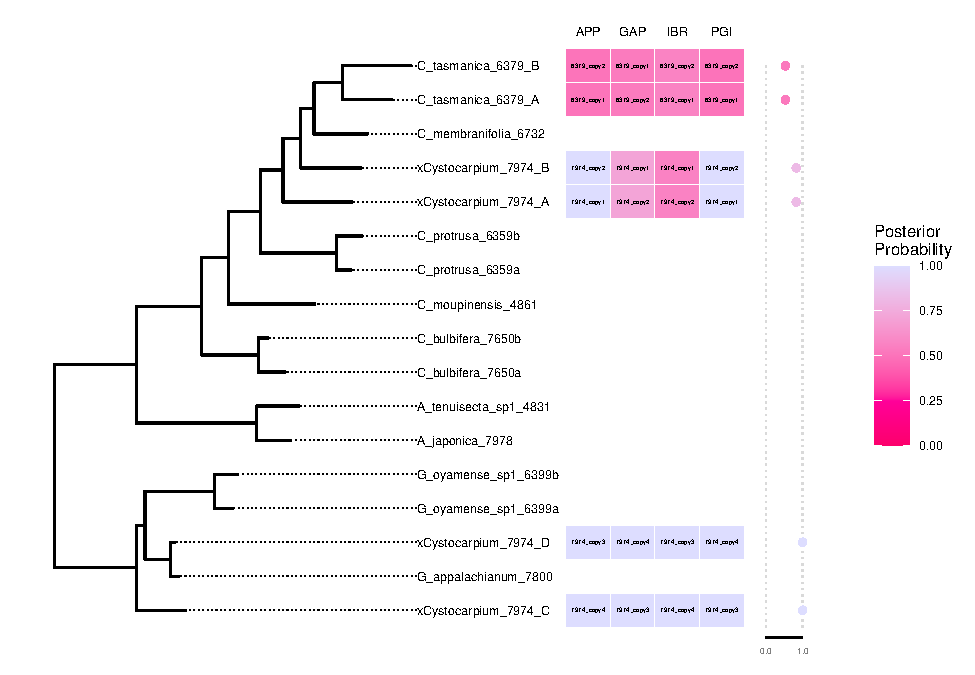
\includegraphics[width=1\linewidth]{_main_files/figure-latex/image7-1} 

}

\caption{Inferred phasing of gene copies into subgenomes summarized on the MAP phylogeny for the Cystopteridaceae dataset}\label{fig:image7}
\end{figure}

\begin{Shaded}
\begin{Highlighting}[]
\FunctionTok{ggsave}\NormalTok{(}\StringTok{\textquotesingle{}../Figures//homologized\_joint\_MAP.pdf\textquotesingle{}}\NormalTok{, }\AttributeTok{height=}\DecValTok{3}\NormalTok{, }\AttributeTok{width=}\DecValTok{7}\NormalTok{)}
\end{Highlighting}
\end{Shaded}

The phase is estimated for the two polyploid accessions xCystocarpium\_7974 and C\_tasmanica\_6379. To the right of the tree, each column represents a locus, and the joint MAP phase assignment is shown as text within each box. Each box is colored by the marginal posterior probability of the phase assignment. These marginal posterior probabilities are useful to quantify the uncertainty within the joint MAP phasing assignment. For example, it may be that the joint MAP phase of a given polyploid has a low marginal posterior probability in some subgenomes but a high marginal posterior probability in other subgenomes. Adjacent to the heatmap is a column that shows the mean marginal probability across loci of the phasing assignment per tip, which summarizes the model's overall confidence in the phasing of that tip.

  \bibliography{book.bib,packages.bib}

\end{document}
